\documentclass[xcolor=dvipsnames]{beamer}

\mode<presentation>
{
  %\usetheme{Frankfurt}
  \usetheme{default}
  % or ...

  \setbeamercovered{transparent}
  % or whatever (possibly just delete it)
  % \setbeamercolor{structure}{bg=canvas, fg=blue}
    \usecolortheme{crane}
  %\usecolortheme[named=Brown]{structure}

}

\usepackage[english]{babel}
\usepackage[utf8x]{inputenc}
%\usepackage[latin1]{inputenc}
\usepackage{times}
\usepackage[T1]{fontenc}
\usepackage{array,booktabs,tabularx}
\newcolumntype{Z}{>{\centering\arraybackslash}X} % centered tabularx columns
\newcommand{\pphantom}{\textcolor{ta3aluminium}} % phantom introduces a vertical space in p formatted table columns??!!
\usepackage{amsmath,amsthm, amssymb, latexsym}
\usepackage{graphicx}
\usepackage{verbatim}

\title[] {Implementación de Arquitectura Mixta de Clasificación de Paquetes Sobre Lógica Reconfigurable.}

\author[] {Jairo N. Trad y Luis R. Romano}


\institute[Universidades] % (optional, but mostly needed)
{
  \scriptsize Laboratorio de Comunicaciones Digitales \\
  \scriptsize Universidad Nacional de Córdoba, Facultad Ciencias Exactas, Físicas y Naturales \\ 
}

\AtBeginSubsection[]
{
  \begin{frame}<beamer>{Agenda}
  %  \scriptsize
    \tiny	
    \tableofcontents[currentsection,currentsubsection]
  \end{frame}
}

% If you wish to uncover everything in a step-wise fashion, uncomment
% the following command: 

%\beamerdefaultoverlayspecification{<+->}

\begin{document}

\begin{frame}
  \titlepage
\end{frame}

\begin{frame}{Agenda}
  \tiny 
  \tableofcontents
  % You might wish to add the option [pausesections]
\end{frame}

\scriptsize

\section{Introducción}

\subsection{Contexto}

\begin{frame}{Introducción}
  \scriptsize
  
  \begin{block}<+->{}

    \begin{itemize}
      \item Las redes de datos crecen en {\bf Complejidad:} nuevas aplicaciones, multimedia.
      \item Crece el volumen de datos y se requiere más velocidad de procesamiento.
      \item {\bf Consolidación} de múltiples servicios sobre redes Ethernet.     
      \item Necesidad de introducir continuas mejoras en el procesamiento de los datos.
      \item Soluciones: no solo rápidas sino también flexibles y escalables.
    \end{itemize}
    
  \end{block}
    

\end{frame}




\begin{frame}{Contexto}
  \begin{block}<+->{Tecnologías de red}  
    \begin{itemize}
      \scriptsize
      \item {\bf Nuevas tendencias} $\rightarrow$ agregación de paquetes en flujos.
      \item Ejemplos: MPLS, VLANs.
      \item MPLS: transporte de datos basado en etiquetas.
      \item VLANs: redes lógicamente independientes conectadas al mismo conmutador físico. 
    \end{itemize}
  \end{block}
  
     \center 
    \newcolumntype{V}{>{\centering\arraybackslash} m{.5\linewidth} }
    \begin{tabularx}{\linewidth}{V|V}

      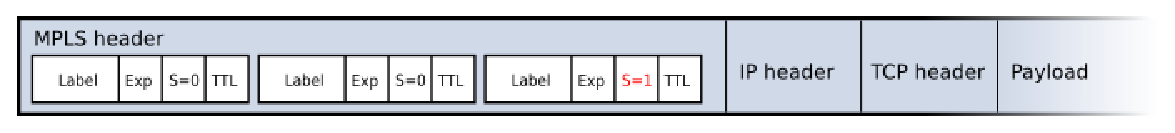
\includegraphics[scale=0.20]{figures/MPLS_packet.eps}
      &
      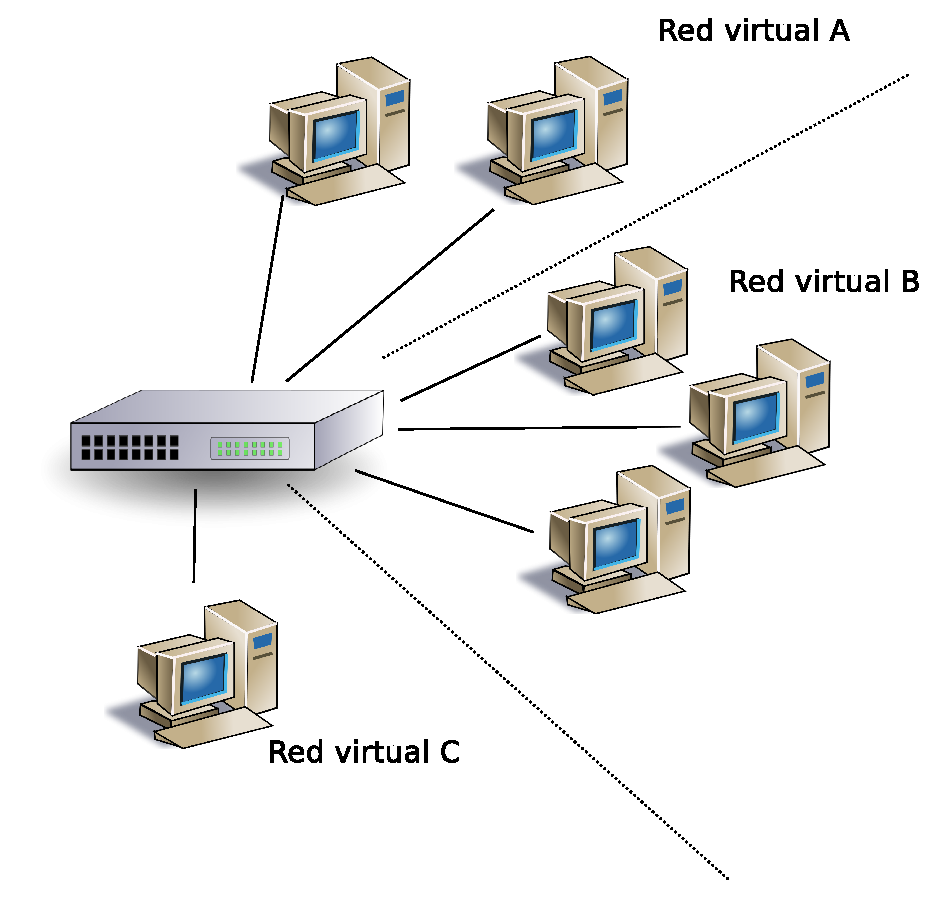
\includegraphics[scale=0.20]{figures/vlan.eps}      
      \\
      \tiny MPLS
      &
      \tiny VLANs
      \\
    \end{tabularx}

\end{frame}  
  


\begin {frame}{Tecnologías Actuales}   
  
  Requerimientos $\rightarrow$ {\bf flexibilidad, performance} 
  
  \begin{block}<+->{Circuitos de Propósito Específico (ASICs)} 
    \begin{itemize}
      \scriptsize
      \item Cientos de bloques especializados trabajando en paralelo
      \item Alto desempeño. No programables, alto costo y tiempo de desarrollo.
    \end{itemize}
  \end{block}

  \begin{block}<+->{Procesadores de Red (NPs)}   
    \begin{itemize}
      \scriptsize
      \item Múltiples elementos de procesamiento, buena performance para ciertas tareas. IXP(Intel), PowerNP (IBM)
      \item Difícil portabilidad, interfaces propietarias
    \end{itemize}
  \end{block}

  \begin{block}<+->{Procesadores de Propósito General (GPPs)} 
    \begin{itemize}
      \scriptsize
      \item Arquitectura PC + Software especializado: \emph{Click}, \emph{Zebra/Xorp/Quagga}
      \item Alta flexibilidad, bajo costo. Limitación por transacciones con RAM y naturaleza secuencial
    \end{itemize}
  \end{block}
  
\end{frame}


\begin{frame}{Nuevas tecnologías}

  \begin{block}<+->{Dispositivos Lógicos Programables (FPGAs)} 
    \begin{itemize}
      \scriptsize
      \item Permiten \emph{reconfiguración} y \emph{reprogramación}, contando con librerías de \emph{Open Hardware}. 
      \item Su performance no es lejana a la de un ASIC. Fabricantes: Altera, Xilinx, Actel.
      \item Incorporación creciente de bloques \emph{hardcore} especializados
    \end{itemize}
    \center
    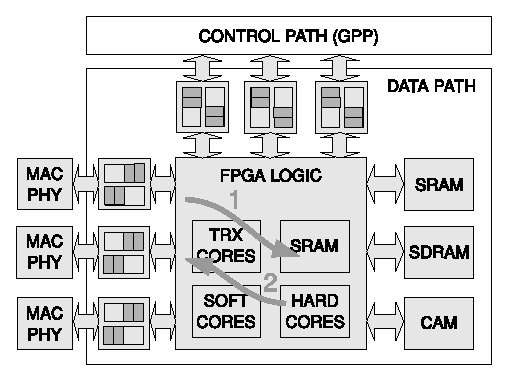
\includegraphics[scale=0.38]{figures/FPGA_based.eps}      
  \end{block}  
\end{frame}

\begin{frame}{FPGA como plataforma para SoC}
  \begin{block}<1->{Sistema en un Chip(SoC)} 
    \begin{itemize}
      \scriptsize
      \item Son circuitos integrados que contienen todo, o la mayoría, de los módulos que componen un sistema informático o electrónico en un solo componente.
	%\item Se diferencian de los microcontroladores en que cuentan con una mayor cantidad de memoria, en general externa, permitiendo ejecutar aplicaciones mas grandes y complejas. 
    \end{itemize}      
  \end{block}

  \begin{block}<2->{FPGA como plataforma para SoC} 
    \begin{itemize}
      \scriptsize
      \item En la ultima década la integración entre FPGAs de propósito general y CPUs tuvo una aceptación amplia como plataforma de para el desarrollo de SoC.    
	\item La flexibilidad, el prototipado rápido, el aumento de la cantidad de lógica reprogramable de propósito general y la creciente disponibilidad de IP cores fueron elementos determinantes que profundizaron esta tendencia.
	\center
        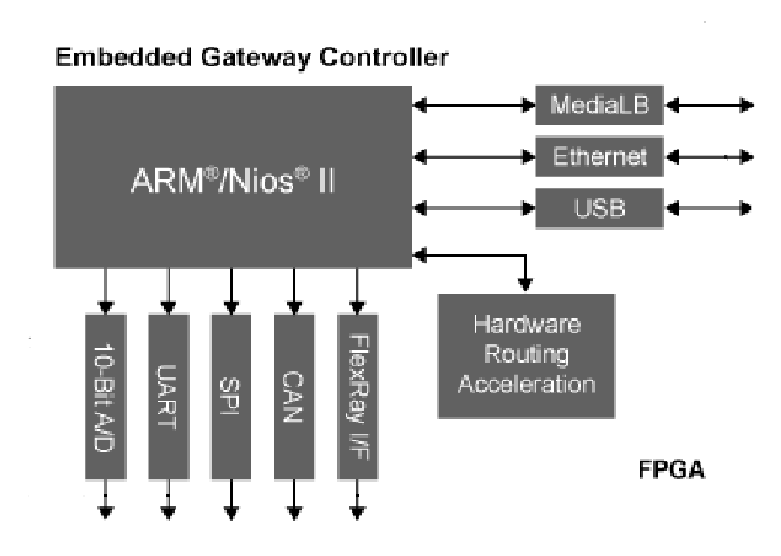
\includegraphics[scale=0.29]{figures/soc2.eps} 

    \end{itemize}      
  \end{block}
\end{frame}


\subsection{Problema marco}

\begin{frame}{Clasificación de Paquetes}

 \begin{block}<+->{Clasificación}   
    \begin{itemize}
      \scriptsize
      \item La necesidad de procesar cada vez más paquetes de datos lleva a lo que se conoce como \textit{clasificación.}
      \item Es el proceso de categorización de paquetes en distintos flujos.
      \item Efectuada en base a un número de campos de una cabecera.
      \item En general, para una clasificación basada en N campos, se dice que la misma es N-dimensional (o multidimensional) 
      \item Un caso en particular de la clasificación unidimensional (N=1) utilizando el campo IP destino es lo que se conoce como \textit{IP Lookup}.     
    \end{itemize}
  \end{block}
\end{frame}

\begin{frame}{Dirección IP - Prefijos}
 \begin{block}<+->{Dirección IP}   
    \begin{itemize}
      \scriptsize
      \item Es un número de 32 bit que identifica un dispositivo dentro de una red que utilice el protocolo IP
      \item Estructura jerárquica. Una parte de la dirección corresponde a la red, y la otra al host dentro de la red
      \item Los bits que corresponden a la parte de red conforman lo que se denomina \textit{prefijo de red}.
     \end{itemize}
  \end{block}
\begin{block}<+->{Formas de representar un prefijo de red}   
    \begin{itemize}
      \scriptsize
      \item Binario con asterisco (132.239 - 1000010011101111*)
      \item Notación A/L, donde A es una dirección IP y L es la longitud del prefijo (132.239.0.0/16)
      \item Notación máscara: se utiliza una dirección de red y una máscara (132.239.0.0 con máscara 255.255.0.0)
     \end{itemize}
  \end{block}
\end{frame}

\begin{frame}{IP LookUp}
 \begin{block}<+->{IP Lookup}   
    \begin{itemize}
      \scriptsize
      \item Se lleva a cabo en el dispositivo de enrutamiento.
      \item Un paquete llega por una interfaz de entrada. Éste porta una dirección IP de destino determinada.
      \item El dispositivo consulta una tabla para determinar la interfaz de salida para el paquete en cuestión
      \item Dicha tabla contiene un conjunto de prefijos con sus correspondientes interfaces de salida.
      \item El paquete es correspondido con el prefijo más largo que esté contenido en la dirección de destino y luego es redirigido  a la correspondiente interfaz de salida
      \item No es una búsqueda trivial, ya que no se busca un valor en particular sino un prefijo contenido dentro de un valor. No aplican los algoritmos de búsqueda tradicionales.   
    \end{itemize}
  \end{block}
\end{frame}

\begin{frame}{Prefijos}
\center 
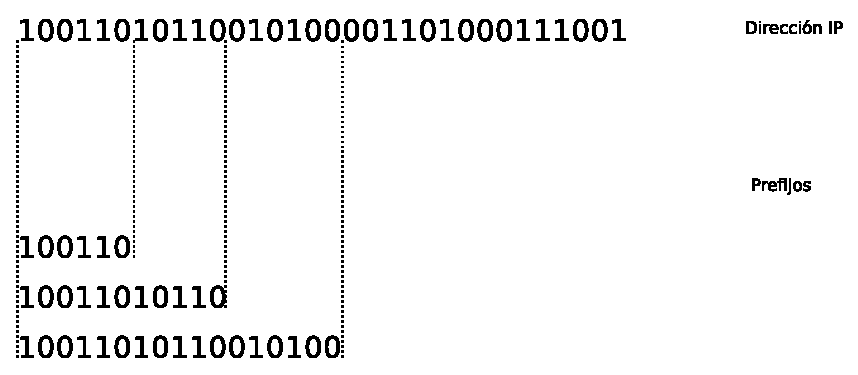
\includegraphics[scale=0.75]{figures/prefijos.eps}
\end{frame}

\subsection{Objetivos}
\begin{frame}{Objetivos}
\begin{block}<+->{Generales}   
    \begin{itemize}
      \scriptsize
      \item Estudiar los diversos algoritmos de clasificación de paquetes para poder encontrar las limitaciones en la implementación de los mismos.
      \item Considerar una plataforma de lógica reprogramable que permita integrar arquitecturas de hardware con software embebido.
    \end{itemize}
  \end{block}
  
\begin{block}<+->{Específicos}   
    \begin{itemize}
      \scriptsize
     	\item Diseñar un sistema embebido que realice la clasificación unidimensional de paquetes mediante una arquitectura mixta, Hardware-Software
	\item Implementar dicho sistema en hardware reconfigurable
	\item Implementar al menos 2 algoritmos conocidos y analizar su performance
	\item Sugerir mejoras en la implementación de los mismos   
    \end{itemize}
  \end{block}
\end{frame}

\section{Sistema}
\subsection{Introducción}
\begin{frame}{Introducción}
\begin{block}<+->{Tipos de soluciones}  
    \begin{itemize}
      \scriptsize
     	\item Soluciones en HW (FPGA, ASIC, NetFPGA)
	\item Soluciones en SW (Click Router)
	\item Complementar las ventajas de ambos mundos 
    \end{itemize}
  \end{block}
  
\center 
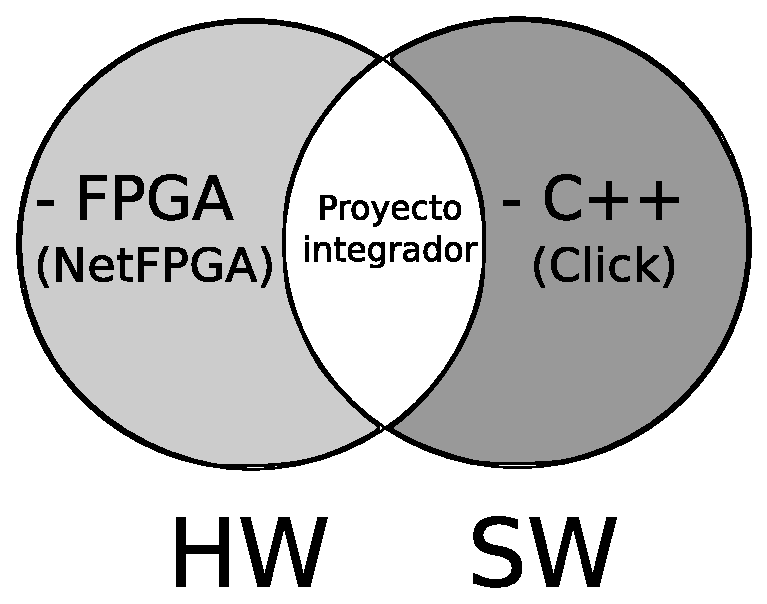
\includegraphics[scale=0.4]{figures/interseccion.eps}
  
\end{frame}
  
\subsection{Solución Propuesta}
\begin{frame}{Solución}

    \begin{enumerate}
      \scriptsize
 \pause     	\item Un flujo de paquetes llega a la interfaz de red del dispositivo y es necesario clasificarlo en distintos flujos para que sea redireccionado.
\pause 	\item Se almacenan en un buffer los paquetes en orden de llegada.
\pause 	\item Se extrae el primer paquete y se toma la información que pertenece a la cabecera, la información completa del paquete queda en espera.
\pause 	\item Se envía al microprocesador la cabecera. 
\pause 	\item El Microprocesador aplica un algoritmo de clasificación a cierta información de la cabecera y reenvía los resultados al Hardware. 
\pause 	\item Se anexa a cada palabra del paquete un Tag adjunto con el resultado de la clasificación y se lo envía hacia la interfaz de salida.
    \end{enumerate}

\end{frame}

\begin{frame}{Arquitectura propuesta}
   \center 
   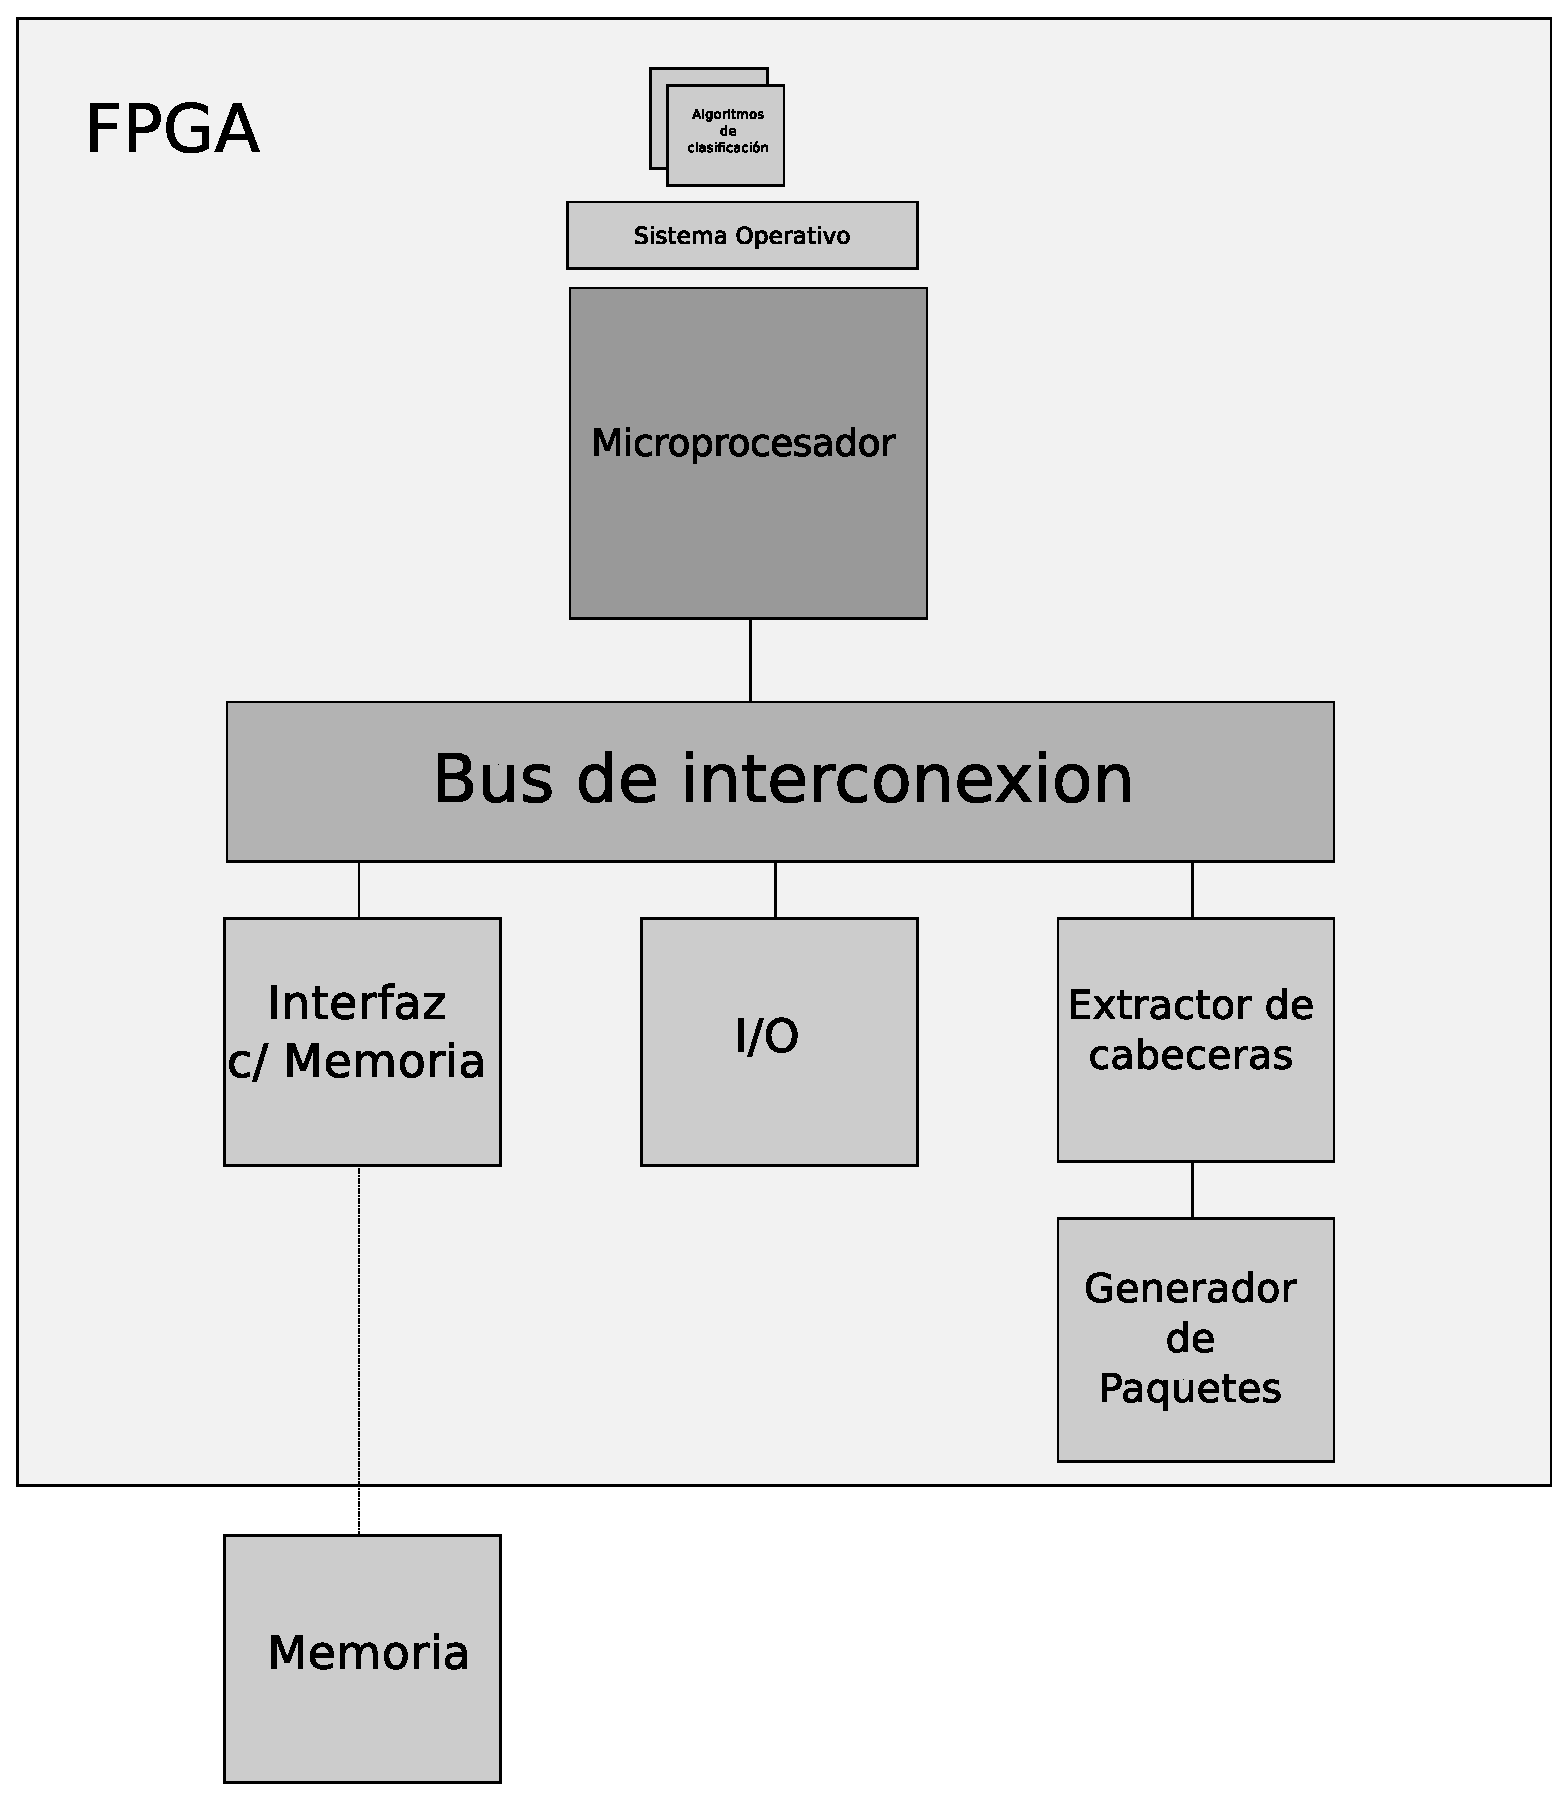
\includegraphics[scale=0.17]{figures/solucion.eps}
\end{frame}

\begin{comment}
\subsection{Descripcion funcional bloque a bloque}
\begin{frame}{Descripcion funcional}
\begin{block}<+->{Microprocesador}   
    \begin{itemize}
      \scriptsize
     	\item Recibe una cabecera y la procesa mediante la ejecución de un software de clasificación de paquetes.
    \end{itemize}
  \end{block}
  \begin{block}<+->{Bus de interconexión}   
    \begin{itemize}
      \scriptsize
     	\item Interconecta los componentes del sistema. 
    \end{itemize}
  \end{block}
\begin{block}<+->{Memoria}   
    \begin{itemize}
      \scriptsize
     	\item Almacena el software de clasificación de paquetes.
    \end{itemize}
  \end{block}
  \begin{block}<+->{Modulo extractor de cabeceras}   
    \begin{itemize}
      \scriptsize
     	\item Extrae una cabecera a partir de cada paquete recibido.
	\item La envía al software de clasificación
	\item Recibe la información generada por dicho software
    \end{itemize}
  \end{block}
\end{frame}
\end{comment}

\subsection{Interfaz de acceso a la cabecera}

\begin{frame}{Interfaz de acceso a la cabecera}

\center 
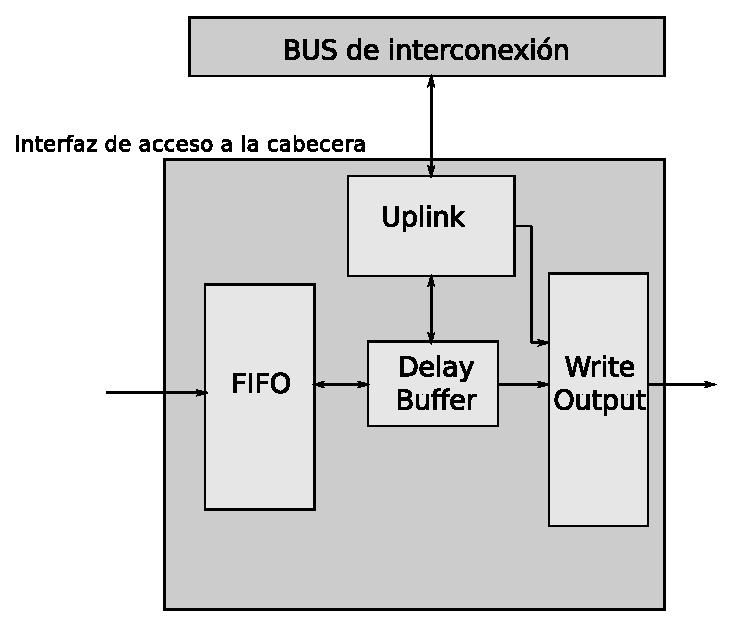
\includegraphics[scale=0.60]{figures/modulo.eps}
\end{frame}

\begin{frame}{Descripción funcional}

\begin{block}<+->{FIFO}   
    \begin{itemize}
      \scriptsize
     	\item Recibe los paquetes y los almacena en una memoria interna.
	\item De tamaño configurable.
    \end{itemize}
  \end{block}
\begin{block}<+->{Delay Buffer}   
    \begin{itemize}
      \scriptsize
     	\item Va tomando los datos desde la FIFO.
	\item Detecta inicio y finalización de cada paquete.
	\item Envía las primeras 5 palabras del paquete, suficientes para cubría la cabecera IP, a Uplink.
	\item Mantiene almacenado el paquete mientras el software toma una decisión.
    \end{itemize}
  \end{block}
\end{frame}
\begin{frame}{Descripción funcional (cont)}
  \begin{block}<+->{Uplink}   
    \begin{itemize}
      \scriptsize
     	\item Entiende las señales que maneja el Bus y puede interrumpir al Procesador.
	\item Genera interrupciones al procesador cuando los datos están disponibles.
	\item Puede enviar al procesador la cabecera completa o solo una parte, siempre en palabras de 32 bits.
	\item Cuando el procesador responde con el resultado de la clasificación, el mismo es almacenado y enviado al módulo Write Output
    \end{itemize}
  \end{block}
\begin{block}<+->{Write Output}   
    \begin{itemize}
      \scriptsize
     	\item Toma la salida de Delay Buffer.
	\item Escribe el resultado que le envía Uplink en la etiqueta que se encuentra anexa en cada una de las palabras del paquete.
    \end{itemize}
  \end{block}
\end{frame}

\subsection{Algoritmos de Clasificación}
\begin{frame}{Algoritmos de Clasificación}
\begin{block}<+->{Linear Lookup (LLU)}   
    \begin{itemize}
      \scriptsize     	
	\item Consiste en una tabla, donde cada entrada contiene un prefijo más un identificador de enlace de salida
	\item Cuando llega un paquete se examina su dirección IP y se va comparando con cada uno de los prefijos almacenados
	\item Debe existir igualdad bit a bit entre el prefijo y la dirección IP
	\item Si esto se cumple para varios prefijos, se opta por el más largo de ellos y el paquete se expide por el enlace asociado a dicho prefijo
	\item Para optimizar este esquema, los prefijos se almacenan en orden decreciente de longitud, de manera que al encontrar una coincidencia no sea necesario seguir buscando en el resto de la tabla
    \end{itemize}
  \end{block}
\end{frame}

\begin{frame}{Algoritmos de Clasificación}
\center 
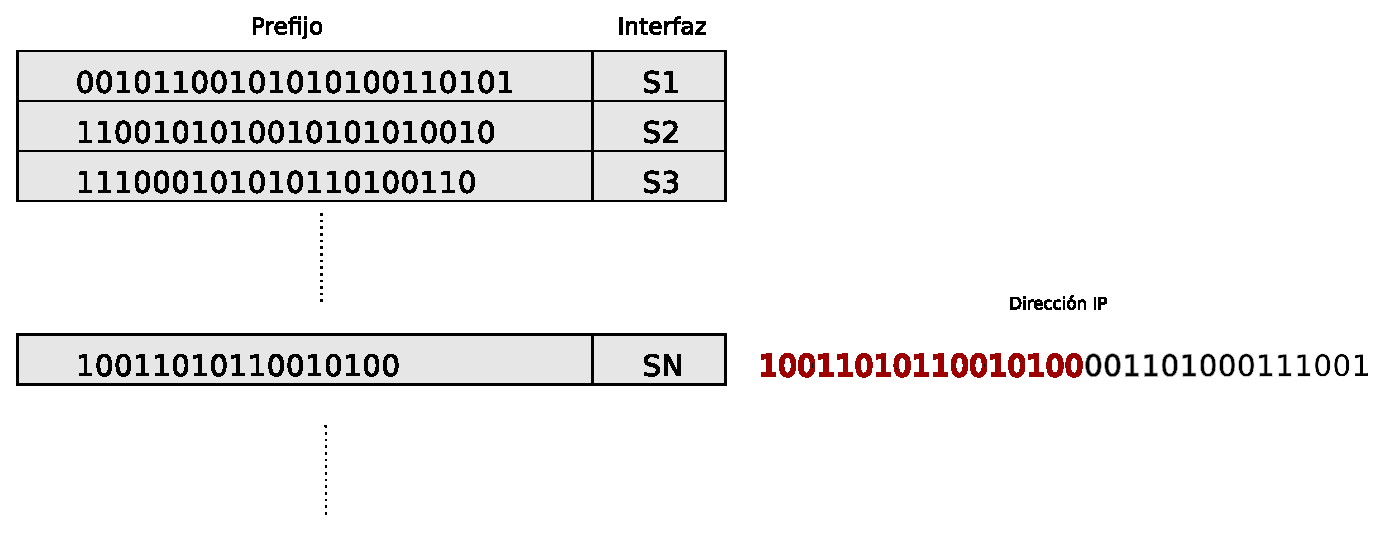
\includegraphics[scale=0.40]{figures/linear.eps}
\end{frame}


\begin{frame}{Algoritmos de Clasificación}
  \begin{block}<+->{Unibit trie lookup (UTL)}   
    \begin{itemize}
      \scriptsize
     	\item Árbol en el cual cada nodo contiene un \textit{puntero-cero }y un \textit{puntero-uno}
	\item Partiendo del nodo raíz, todos los prefijos que comienzan con 0 son almacenados en el subárbol apuntado por el puntero-cero y aquellos que comienzan con 1 se almacenan en el subárbol apuntado por el puntero-uno.
	\item Cada subárbol es construido recursivamente de manera similar usando los bits restantes de cada uno de los prefijos
    \end{itemize}
  \end{block}
\end{frame}

\begin{frame}{Algoritmos de Clasificación}
  \begin{block}<+->{Ejemplo}   
	\begin{center}
	\begin{tabular}{|c|c|} \hline
		\textbf{Prefijo} & \textbf{Enlace de salida} \\ \hline
		101* & S1 \\
		111* & S2 \\
		11001* & S3 \\
		1* & S4 \\
		0* & S5 \\
		1000* & S6 \\
		100000* & S7 \\
		100* & S8 \\
		110* & S9 \\	\hline
	\end{tabular}	
\end{center}

  \end{block}
\end{frame}

\begin{frame}{Algoritmos de clasificación}
\center 
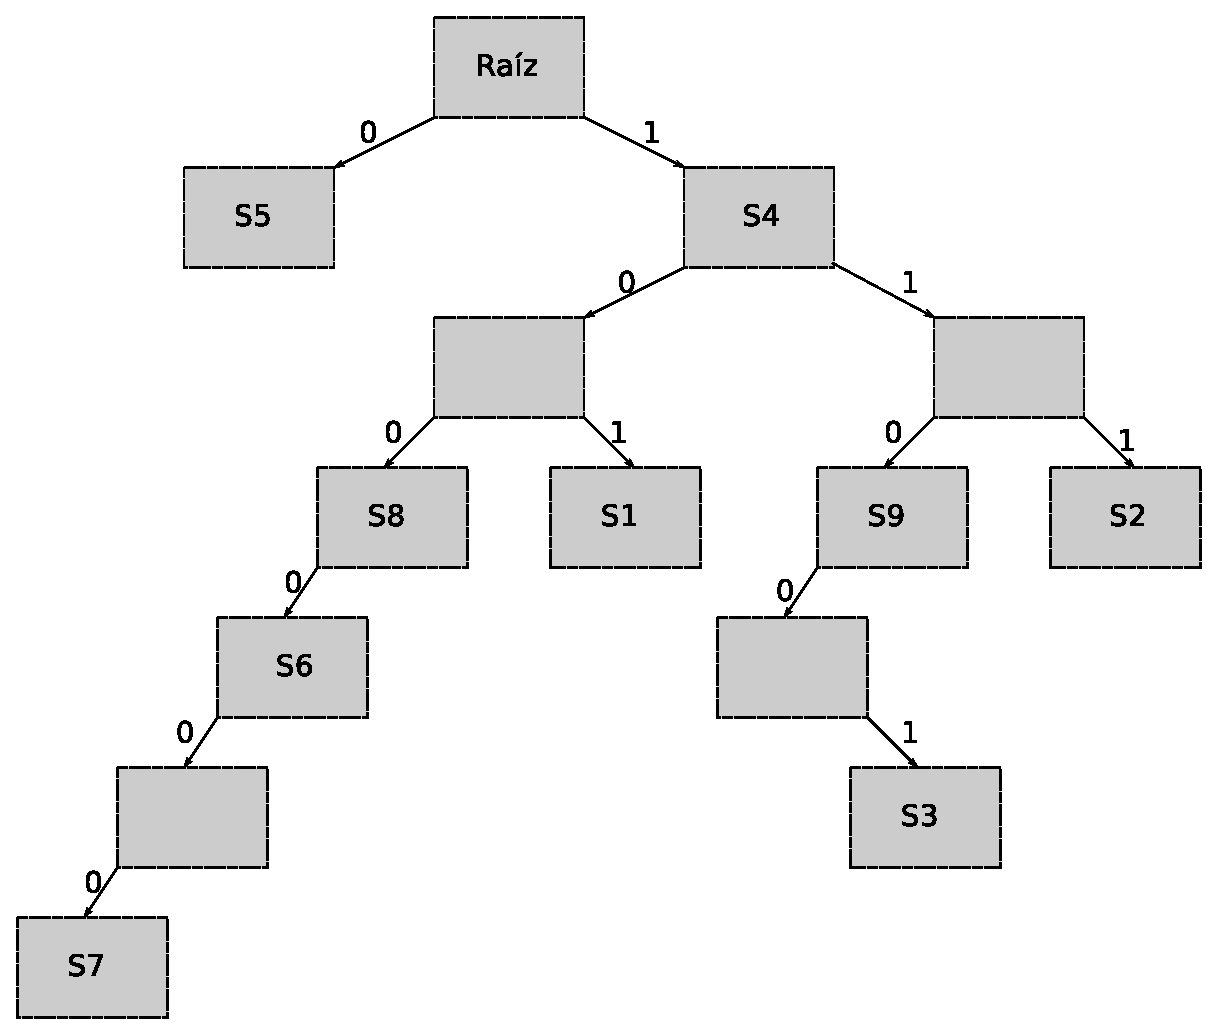
\includegraphics[scale=0.40]{figures/trie.eps}
\end{frame}

\section{Hardware}

\subsection{Formato de la palabra}
\begin{frame}{Formato de la palabra}

\center 
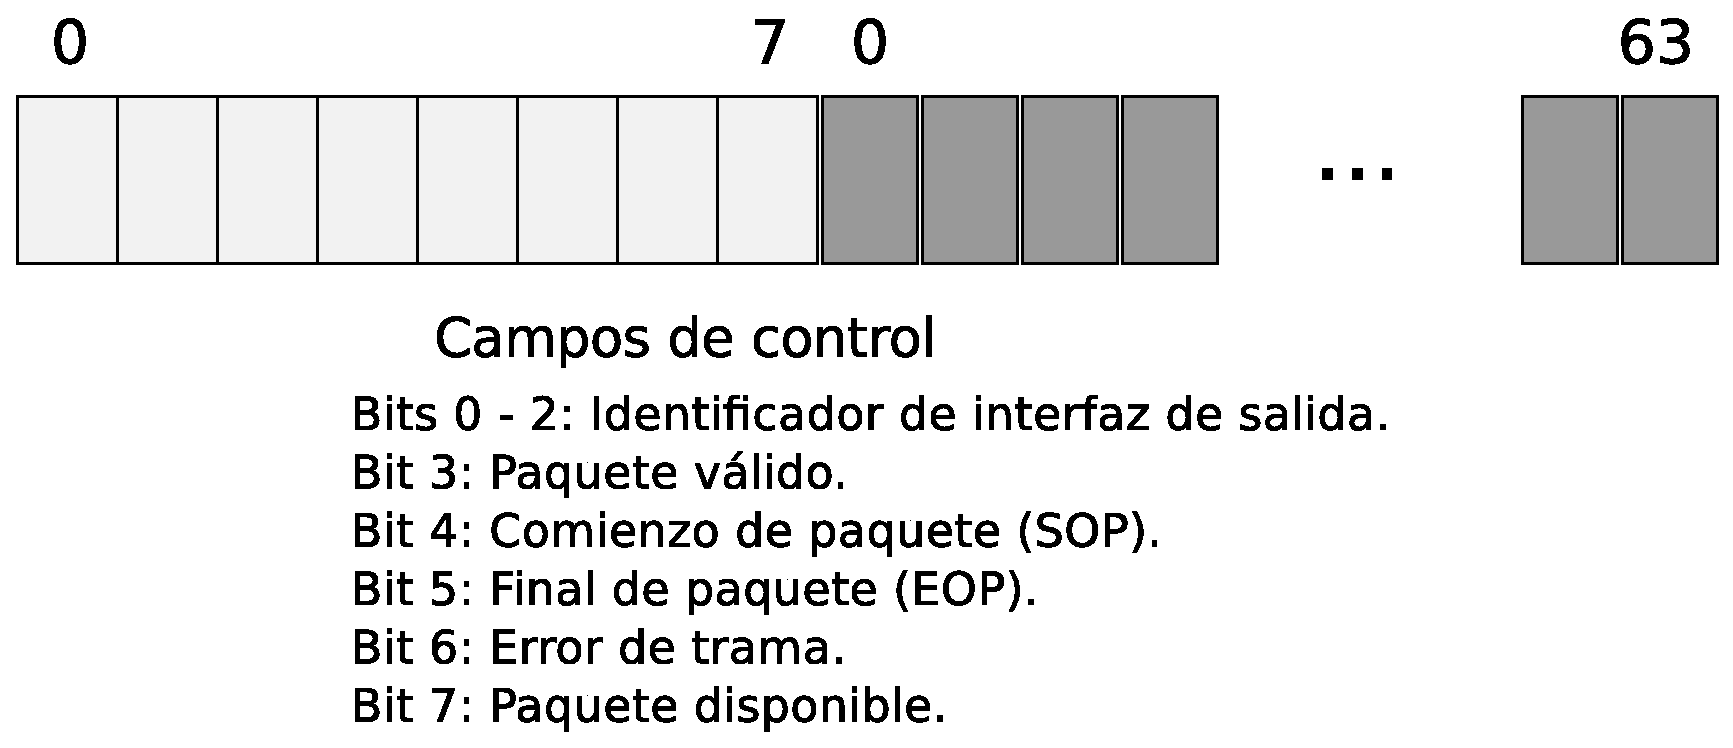
\includegraphics[scale=0.35]{figures/datocontrol.eps}

\end{frame}

\subsection{Etapas del sistema}
\begin{frame}{Etapas}

\center 
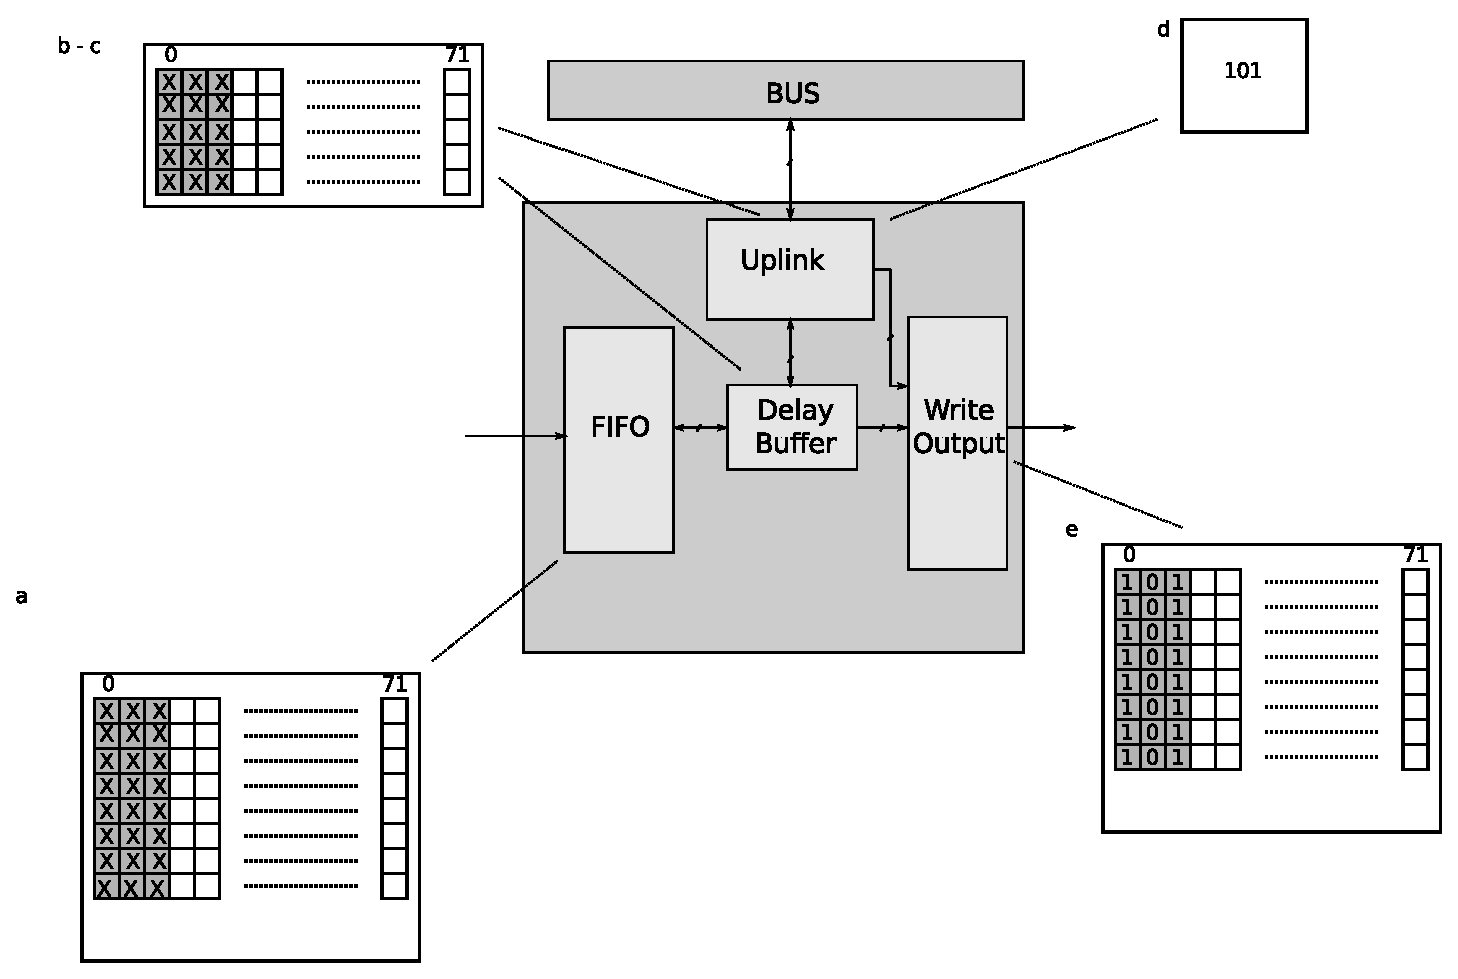
\includegraphics[scale=0.35]{figures/moduloexp.eps}

\end{frame}

\subsection{Diagrama en bloques: Lineas E/S}

\begin{frame}{Generador}
  \begin{block}<+->{Generador}
	\begin{itemize}
      \scriptsize
	\item Permite iniciar la generación de paquetes desde un interruptor externo
	\item Es posible parametrizar la distancia, en ciclos de clock, entre la generación de un paquete y el siguiente.
	\item Puede generar una cantidad variable de paquetes, con valores diferentes en todos sus campos.
	\item Mantiene un contador global de la cantidad de paquetes generados y lo imprime en la ultima palabra del Payload de cada uno.
	\center
	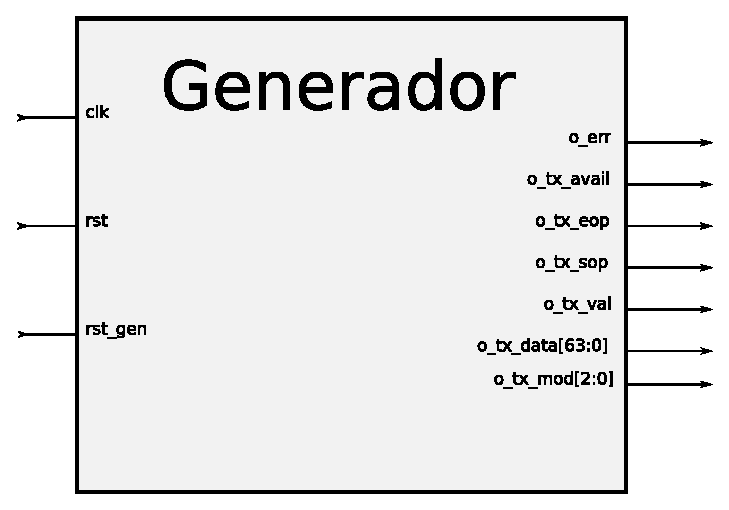
\includegraphics[scale=0.40]{figures/bloqgenerador.eps}
	   \end{itemize}
\end{block}

\end{frame}

\begin{frame}{FIFO}
  \begin{block}<+->{FIFO}
	\begin{itemize}
      \scriptsize
	\item Se trata de una FIFO estándar, adaptada de un codigo disponible en Opencores.
	\item Almacena palabras de 72 bits, 64 de la palabra correspondiente al paquete y 8  bits de control.
	\item Es posible parametrizar la cantidad de palabras, en potencias de 2, que esta FIFO almacena.
	\center
	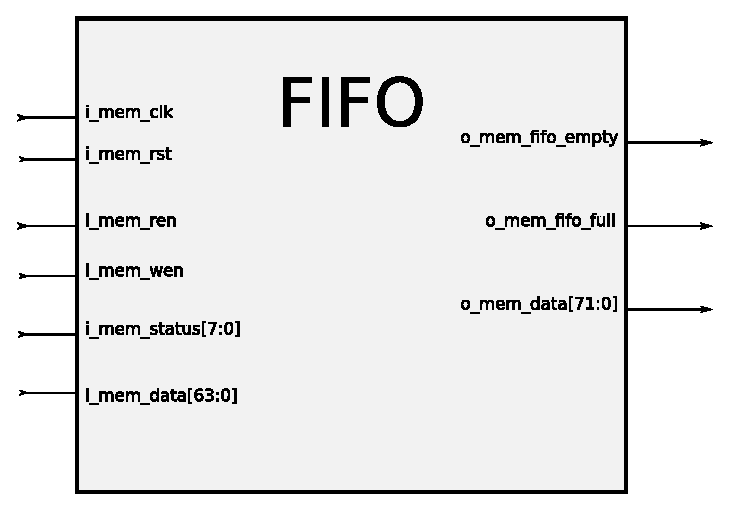
\includegraphics[scale=0.40]{figures/bloqfifo.eps}
	   \end{itemize}
\end{block}

\end{frame}


\begin{frame}{Delay Buffer}
 \begin{block}<+->{Delay Buffer}
	\begin{itemize}
      \scriptsize
	\item Desarrollado íntegramente para este proyecto.
	\item Registro de desplazamiento de 8 posiciones de 72 bits.
	\item Detecta la llegada de un paquete a la FIFO, carga 5 palabras (cabecera) y envía una copia a Uplink.
	\item Cuando el software termina la clasificación, continúa leyendo la FIFO y transfiere el resto del paquete.
	\item Implementación basada en máquina de estados.

	   \end{itemize}
\end{block}

\end{frame}

\begin{frame}{Delay Buffer}
 \begin{tabularx}{\linewidth}{Z|Z}
    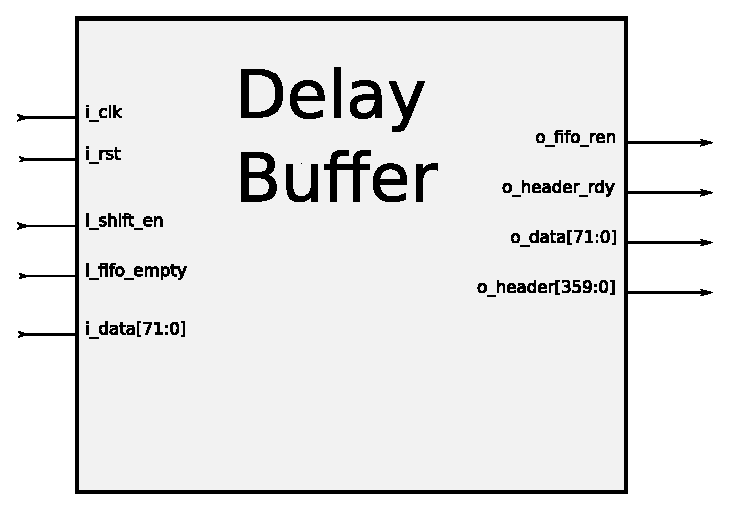
\includegraphics[scale=0.40]{figures/bloqdelaybuffer.eps} 
    &
    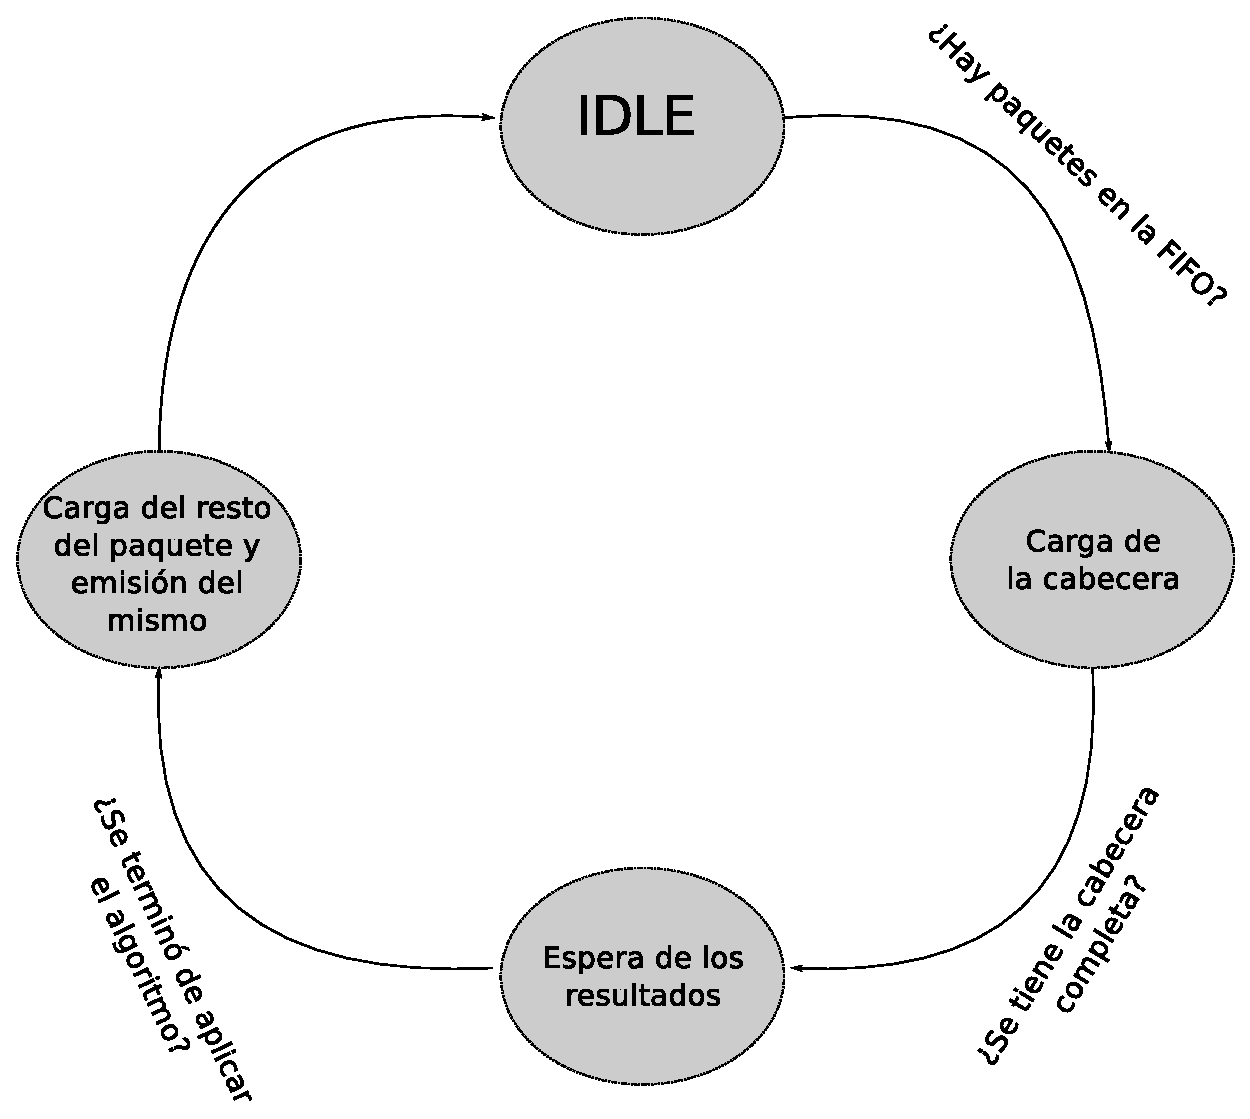
\includegraphics[scale=0.25]{figures/estdelay.eps}
    \\
  \end{tabularx}

\end{frame}

\begin{frame}{Delay Buffer}

\center 

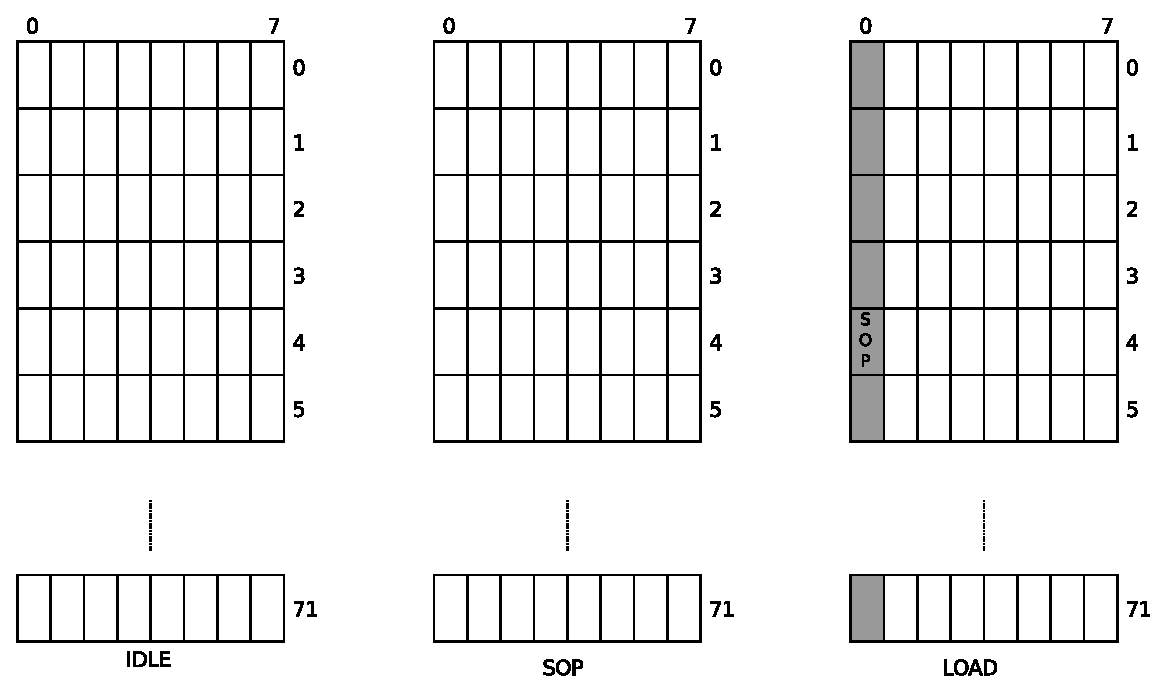
\includegraphics[scale=0.50]{figures/regdespl01.eps}

\end{frame}

\begin{frame}{Delay Buffer}

\center 

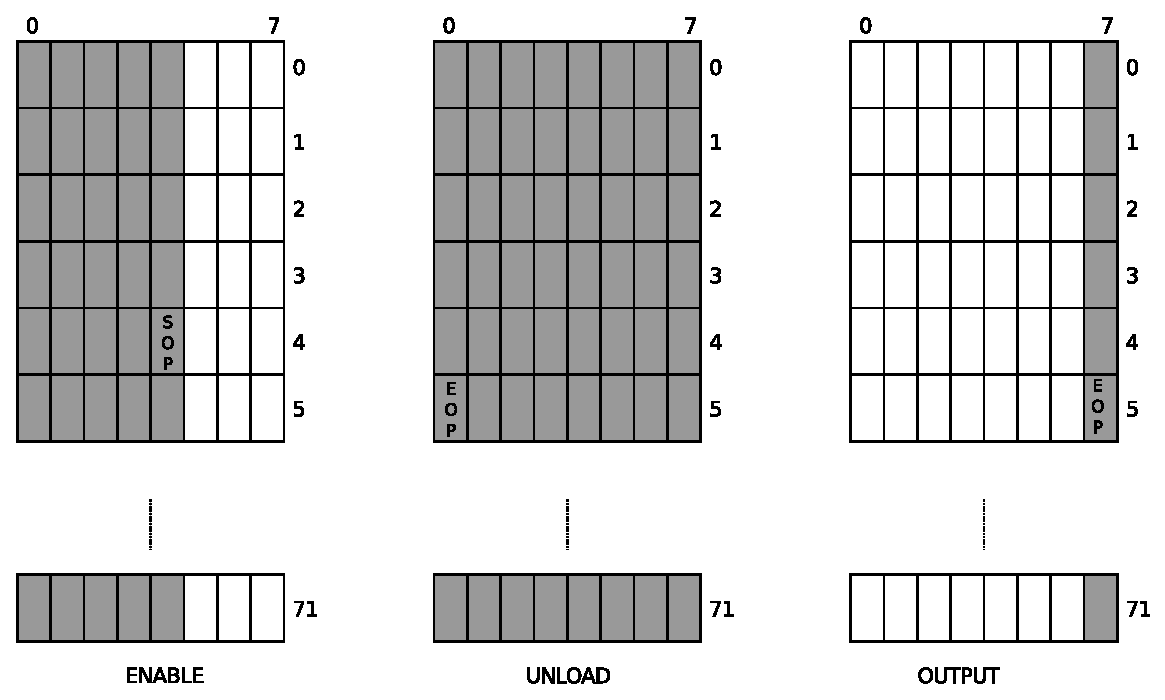
\includegraphics[scale=0.50]{figures/regdespl02.eps}

\end{frame}

\begin{frame}{Uplink}
 \begin{block}<+->{Uplink}
	\begin{itemize}
      \scriptsize
	\item Gestiona la comunicación entre el procesador y el resto de los componentes.
	\item Configurado para trabajar con las señales del bus Avalon.
	\item 2 Versiones: Una transfiere cabecera completa y la otra sólo la dirección IP de destino.
	
	   \end{itemize}
\end{block}
\end{frame}

\begin{frame}{Uplink}
 \begin{tabularx}{\linewidth}{Z|Z}
    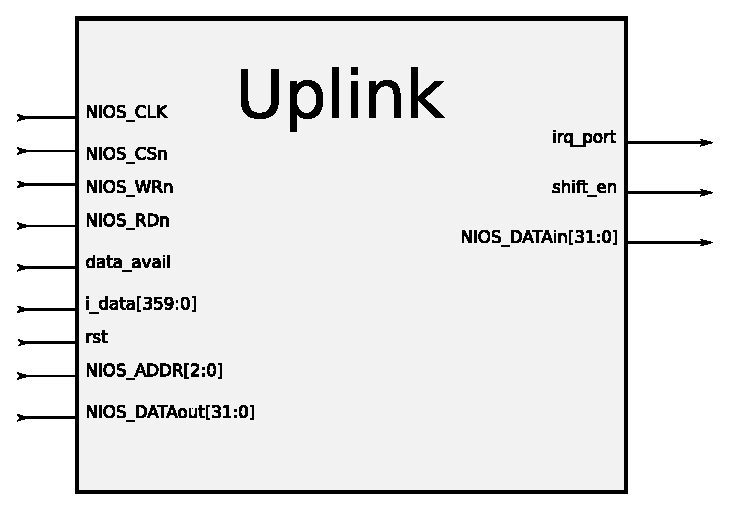
\includegraphics[scale=0.40]{figures/bloquplink.eps} 
    &
    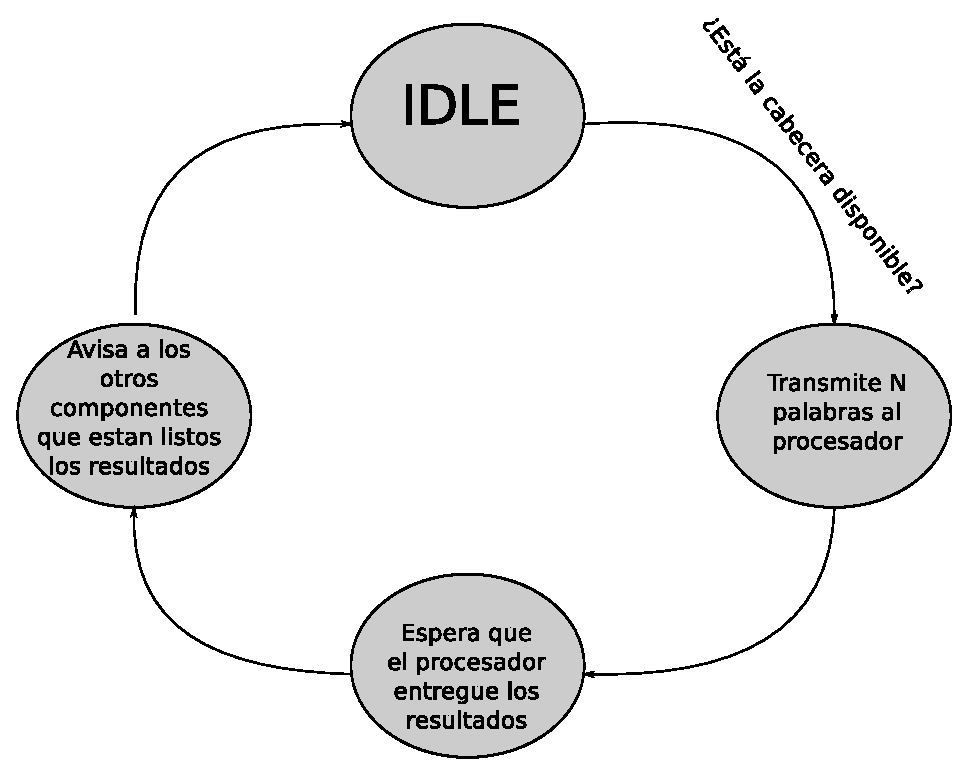
\includegraphics[scale=0.35]{figures/estuplink.eps}
    \\
  \end{tabularx}
\end{frame}

\begin{frame}{Uplink}
  \begin{block}<+->{Uplink}
	\begin{itemize}
      \scriptsize
	\item La primera versión de Uplink transfiere al microprocesador toda la cabecera completa en 15 palabras de 32 bits. 
	\center
	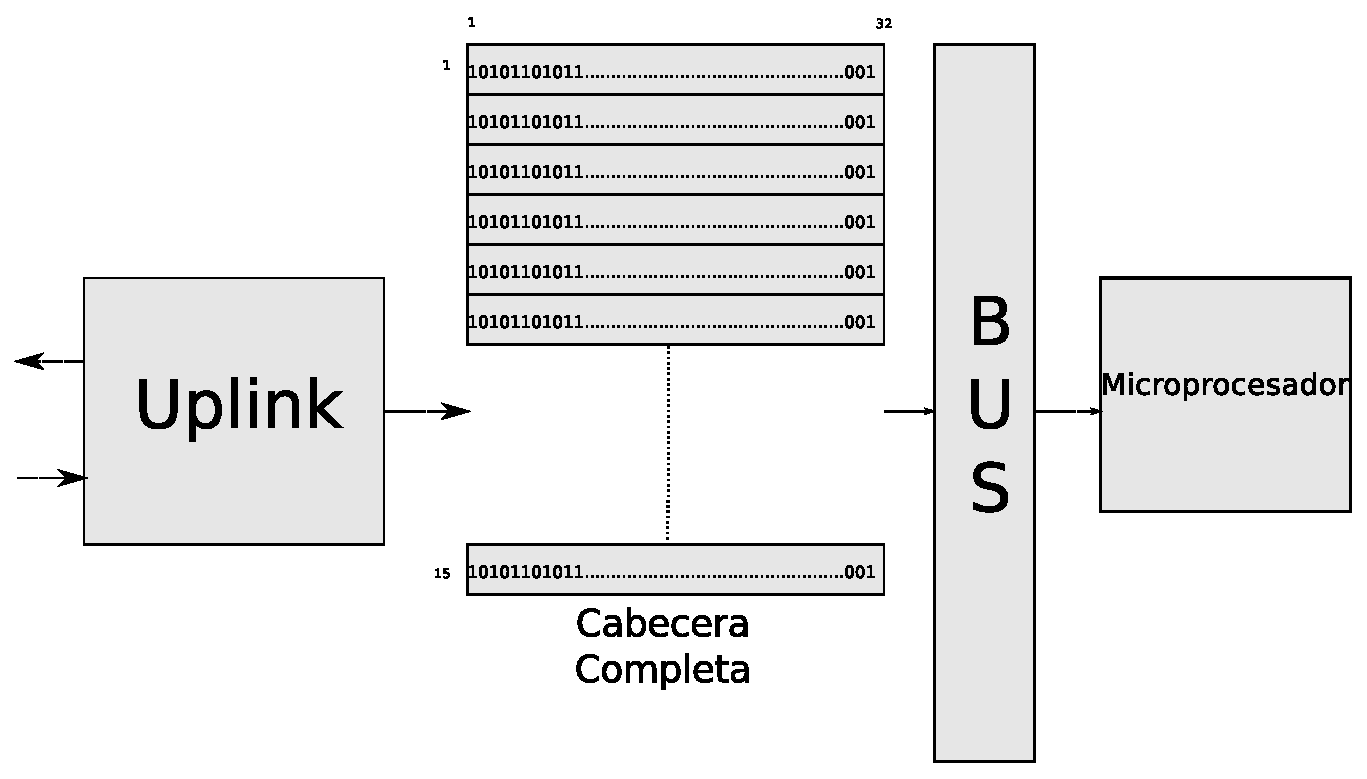
\includegraphics[scale=0.20]{figures/15pal.eps}  
	   \end{itemize}
	\begin{itemize}
      \scriptsize
	\item La segunda versión de Uplink transfiere al microprocesador solo la dirección IP destino en una palabra de 32 bits.
	\center
	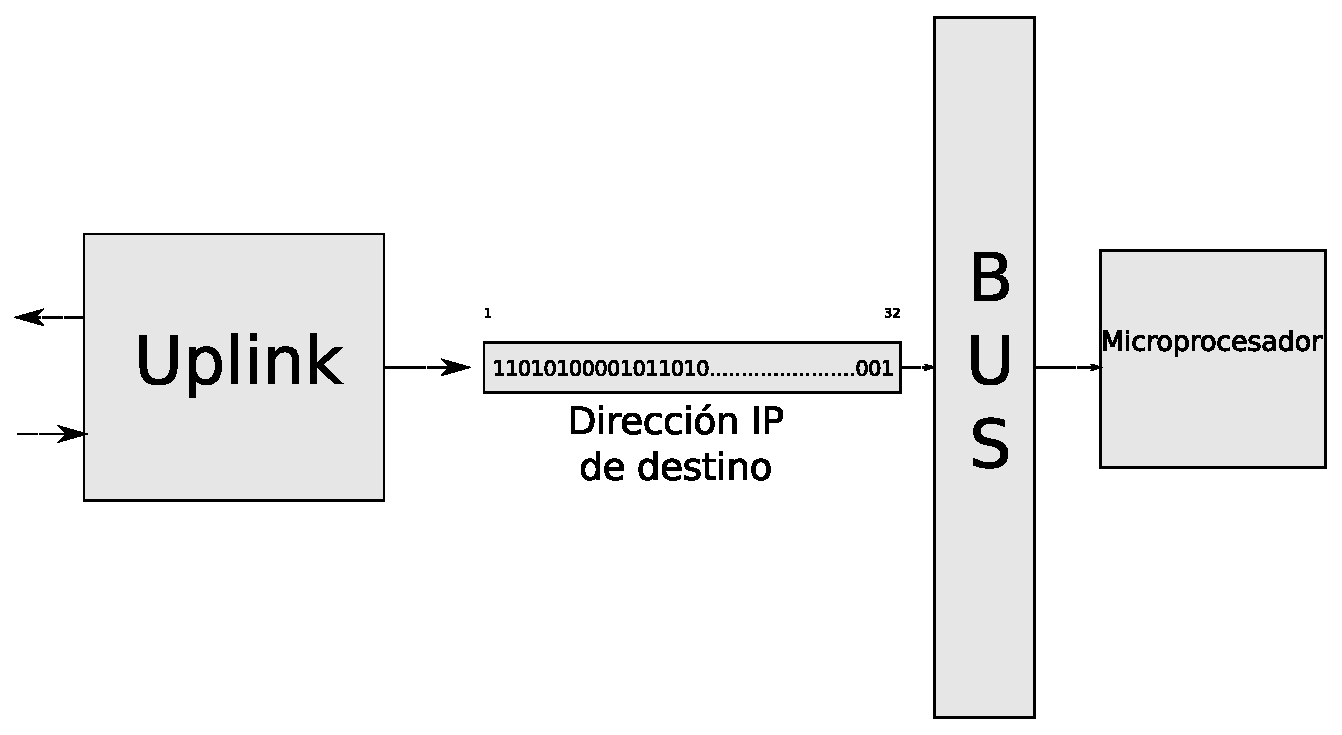
\includegraphics[scale=0.20]{figures/1pal.eps}
   \end{itemize}
\end{block}
\end{frame}

\begin{frame}{Write Output}
 \begin{block}<+->{Write Output}
	\begin{itemize}
      \scriptsize
	\item Toma el resultado emitido por el microprocesador y lo coloca en los campos de control correspondientes.	
	   \end{itemize}
	   \center 
 \begin{tabularx}{\linewidth}{Z|Z}
    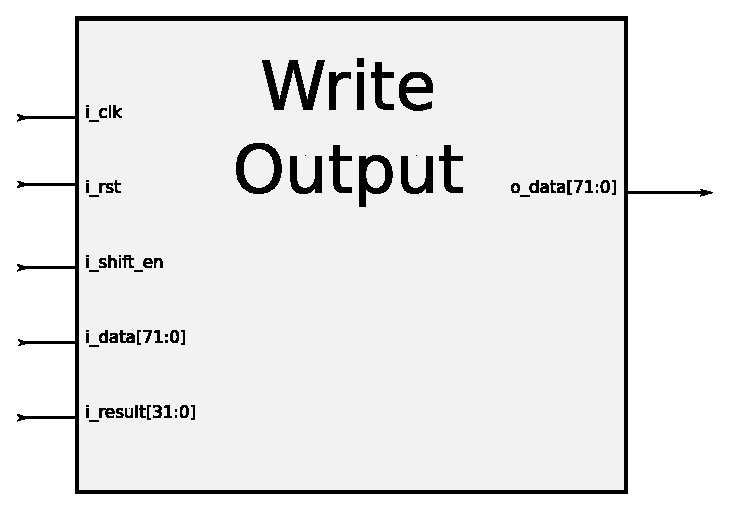
\includegraphics[scale=0.40]{figures/bloqwrite.eps} 
    &
    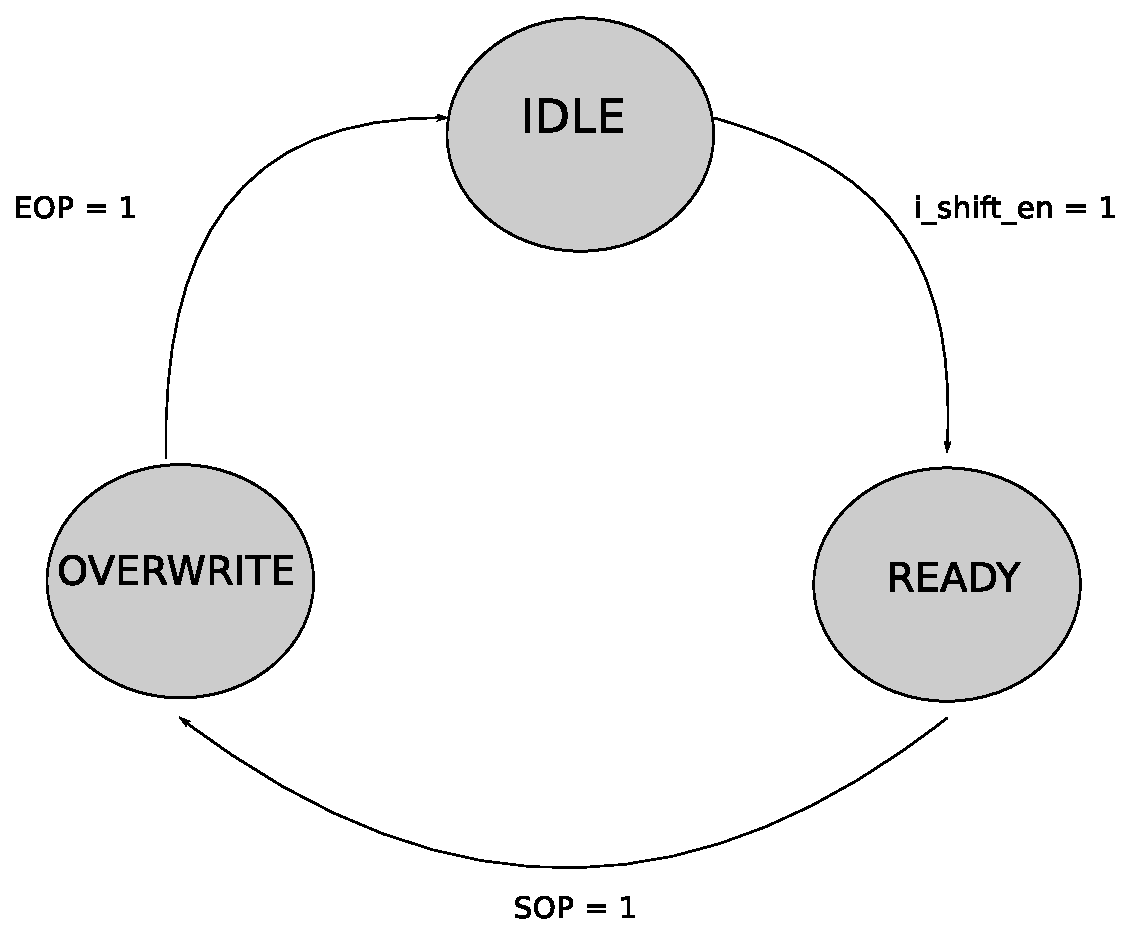
\includegraphics[scale=0.25]{figures/estwritecompleto.eps}
    \\
  \end{tabularx}
\end{block}
\end{frame}


\section{Software}
%\subsection{Introducción}

\begin{frame}{Introducción}
 \begin{block}<+->{Software}
	\begin{itemize}
      \scriptsize
	\item Busqueda Lineal (LLU)
	\item Busqueda en Arbol
	\item C++ (STL container)	
	   \end{itemize}
\end{block}
\end{frame}



\subsection{Algoritmos}
\begin{frame}{Algoritmos}
\begin{block}<+->{LLU}   
    \begin{itemize}
      \scriptsize
     	
     	\item Template \emph{list}
     	\item Cada nodo tiene 3 campos: Dirección de red, Máscara de red e Identificador de decisión
	\item Lista ordenada en base a longitud de máscara de red. Se recorre con un iterador
	\item En cada iteración, Realiza un AND con el valor de máscara del nodo que está siendo apuntado
	\item Si el resultado de la operación es igual al valor de dirección de red de dicho nodo, entonces se retorna con el valor identificador de decisión
	\item En otro caso, continúa la búsqueda en el siguiente nodo
    \end{itemize}
  \end{block}
\end{frame}

\begin{frame}{Algoritmos - LLU}
\begin{block}<+->{iproute}   
    \begin{itemize}
      \scriptsize
     	\item unsigned int addr
     	\item unsigned int mask
     	\item unsigned int gw
    \end{itemize}
  \end{block}

\begin{block}<+->{iplookup}   
    \begin{itemize}
      \scriptsize
     	\item list<iproute> table
	\item void order()
	\item int addEntry (unsigned int addr, unsigned int mask, int gw)
	\item unsigned int showGateway (unsigned int addr)
    \end{itemize}
  \end{block}
\end{frame}
	
\begin{frame}{Algoritmos}

	\center	
	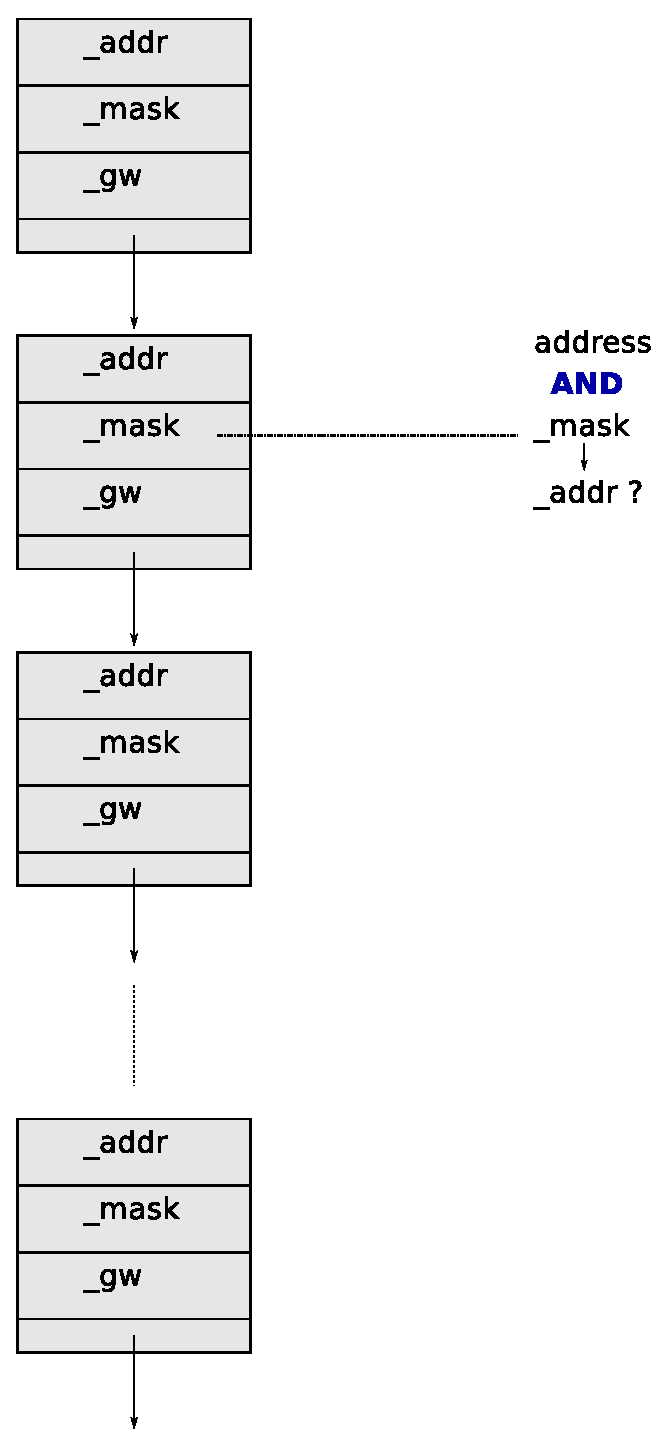
\includegraphics[scale=0.30]{figures/lluimp.eps}  

\end{frame}

\begin{frame}{Algoritmos}
\begin{block}<+->{UTL}   
    \begin{itemize}
      \scriptsize
     	
     	\item Se implementaron clases propias, donde se definieron las características de los nodos del árbol, como así también las operaciones de inserción y búsqueda
     	\item Nodo \emph{común} y nodo \emph{decisión}
	\item Cada nodo tiene 2 campos: \emph{gw} y \emph{zero / one}
	\item El algoritmo de búsqueda toma como entrada la dirección IP de destino del paquete a clasificar
	\item Testeo bit a bit de la misma, partiendo con un puntero de recorrido desde el nodo raíz
	\item Si el bit de la dirección es 0 y el puntero \emph{zero} está apuntando hacia algún nodo, el puntero de recorrido se mueve al nodo apuntado por el puntero zero
	\item En caso contrario, se mueve al nodo apuntado por el puntero \emph{one} (En caso de que exista alguno).
	\item El puntero de recorrido puede quedar en un nodo común o en un nodo decisión
	\item En cada iteración se debe guardar el valor de gw en caso de tratarse de un nodo decisión
	\item Ruta por defecto: nodo raiz
    \end{itemize}
  \end{block}
\end{frame}


\begin{frame}{Algoritmos - UTL}
\begin{block}<+->{trienode}   
    \begin{itemize}
      \scriptsize
     	\item int id;
     	\item PtrTrienode zero;
     	\item PtrTrienode one;
    \end{itemize}
  \end{block}

\begin{block}<+->{trie}   
    \begin{itemize}
      \scriptsize
     	\item PtrTrienode root;
	\item PtrTrienode actual;
	\item PtrTrienode padre;
	\item void insert (unsigned int netAddress, unsigned int mask, int id)
	\item int search (unsigned int address)
    \end{itemize}
  \end{block}
\end{frame}	


\begin{frame}{Algoritmos}

	\center	
	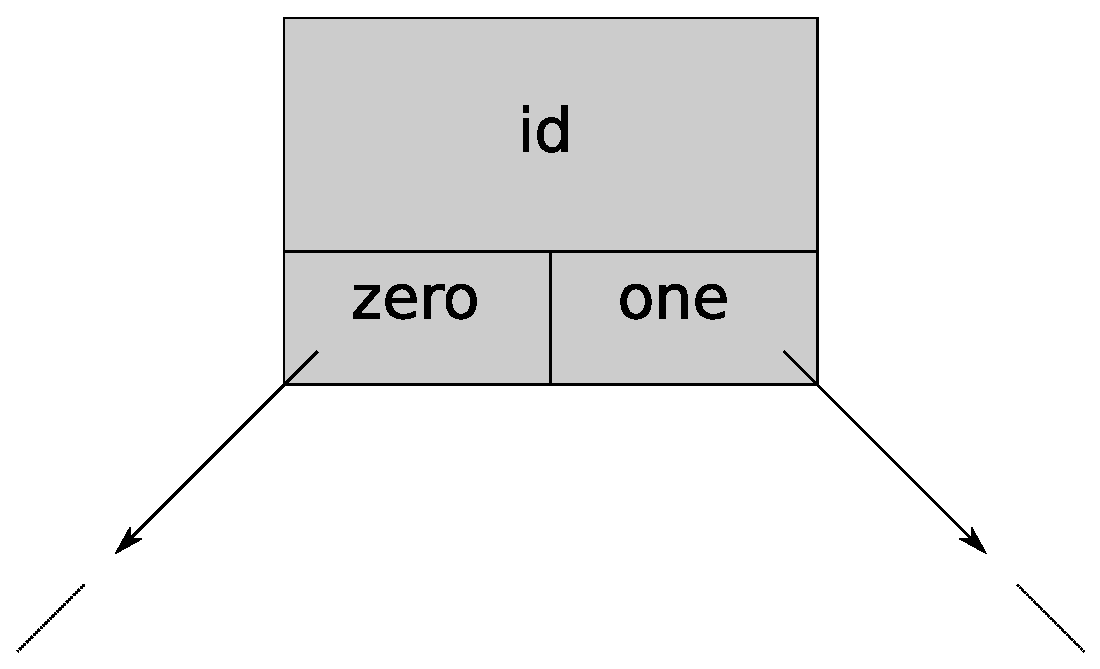
\includegraphics[scale=0.50]{figures/utlimp.eps}  

\end{frame}

\begin{frame}{Ejemplo inserción} 
\center	
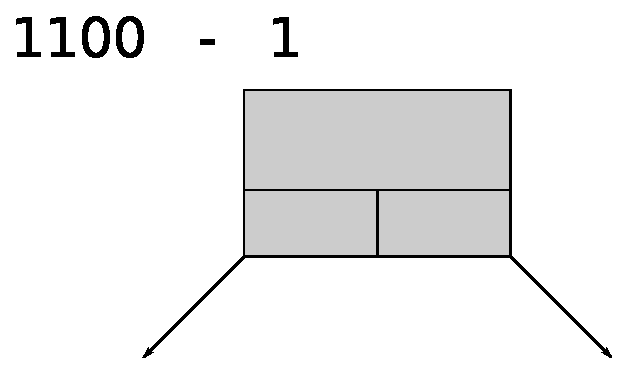
\includegraphics[scale=0.30]{figures/lluinsert01.eps} 
\end{frame}

\begin{frame}{Ejemplo inserción} 
\center	
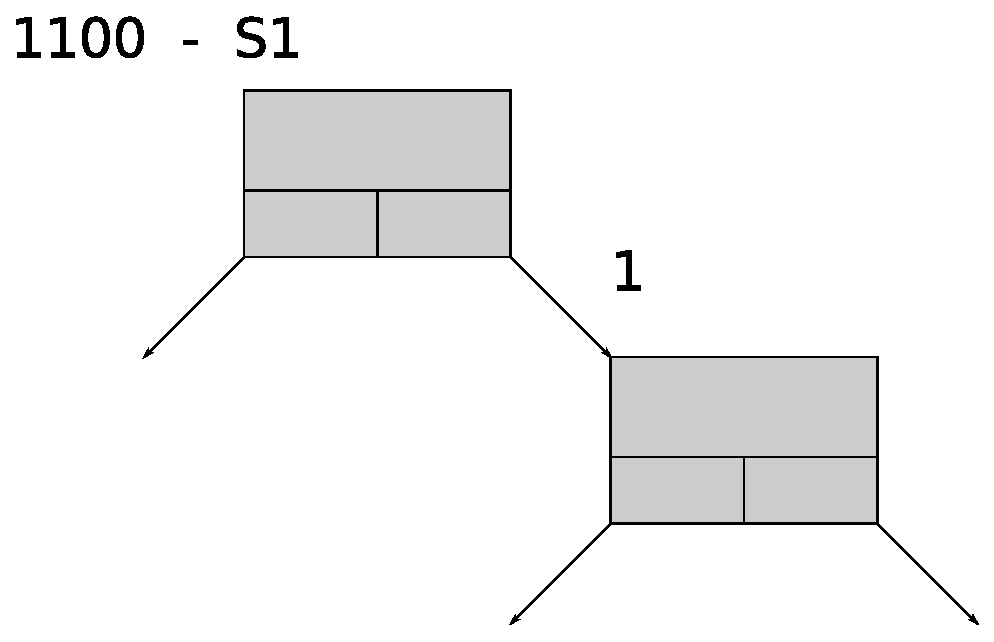
\includegraphics[scale=0.30]{figures/lluinsert02.eps} 
\end{frame}

\begin{frame}{Ejemplo inserción} 
\center	
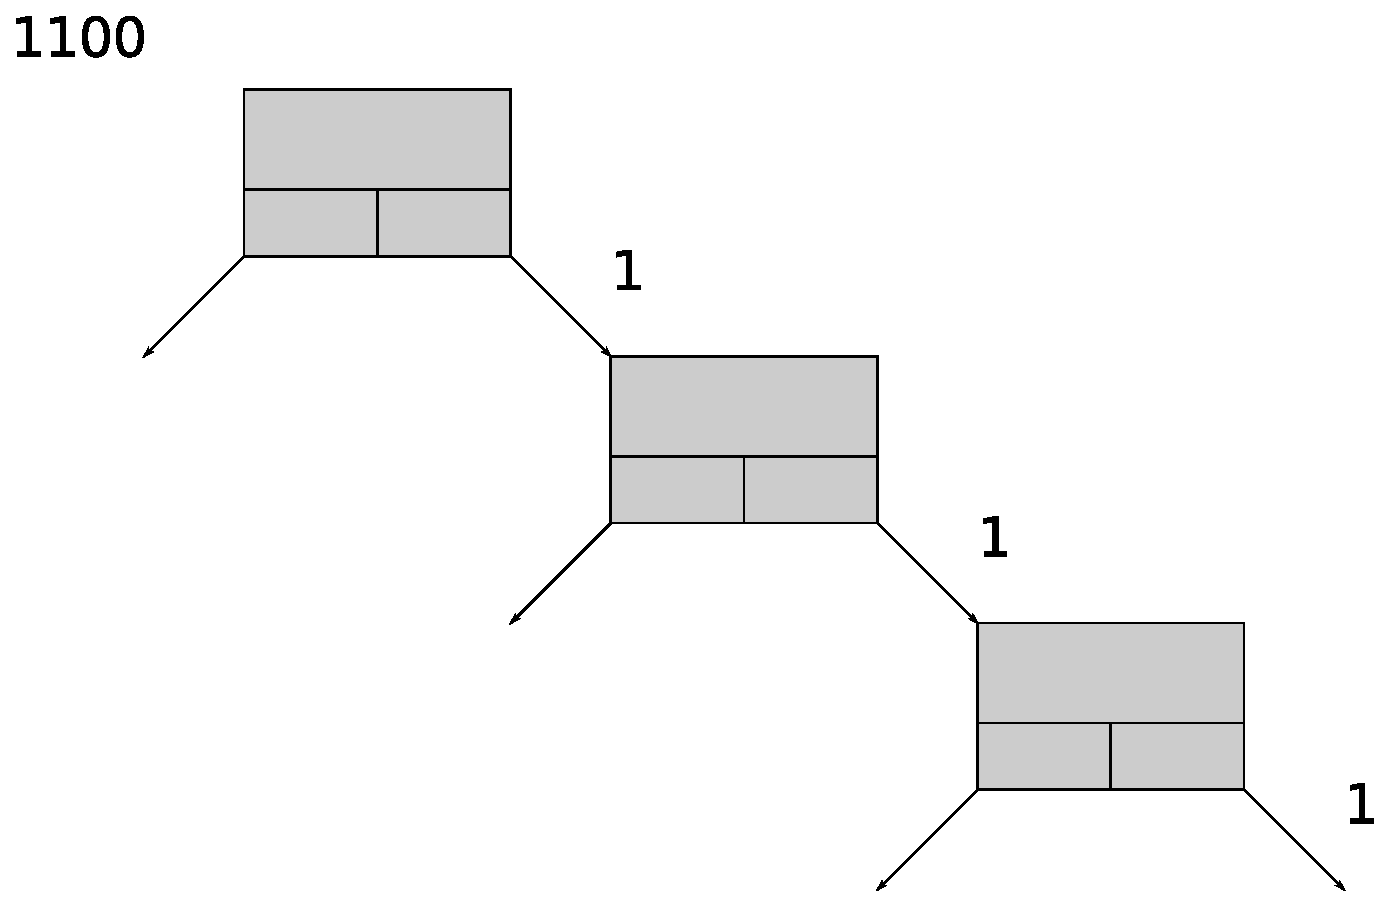
\includegraphics[scale=0.30]{figures/lluinsert03.eps} 
\end{frame}

\begin{frame}{Ejemplo inserción} 
\center	
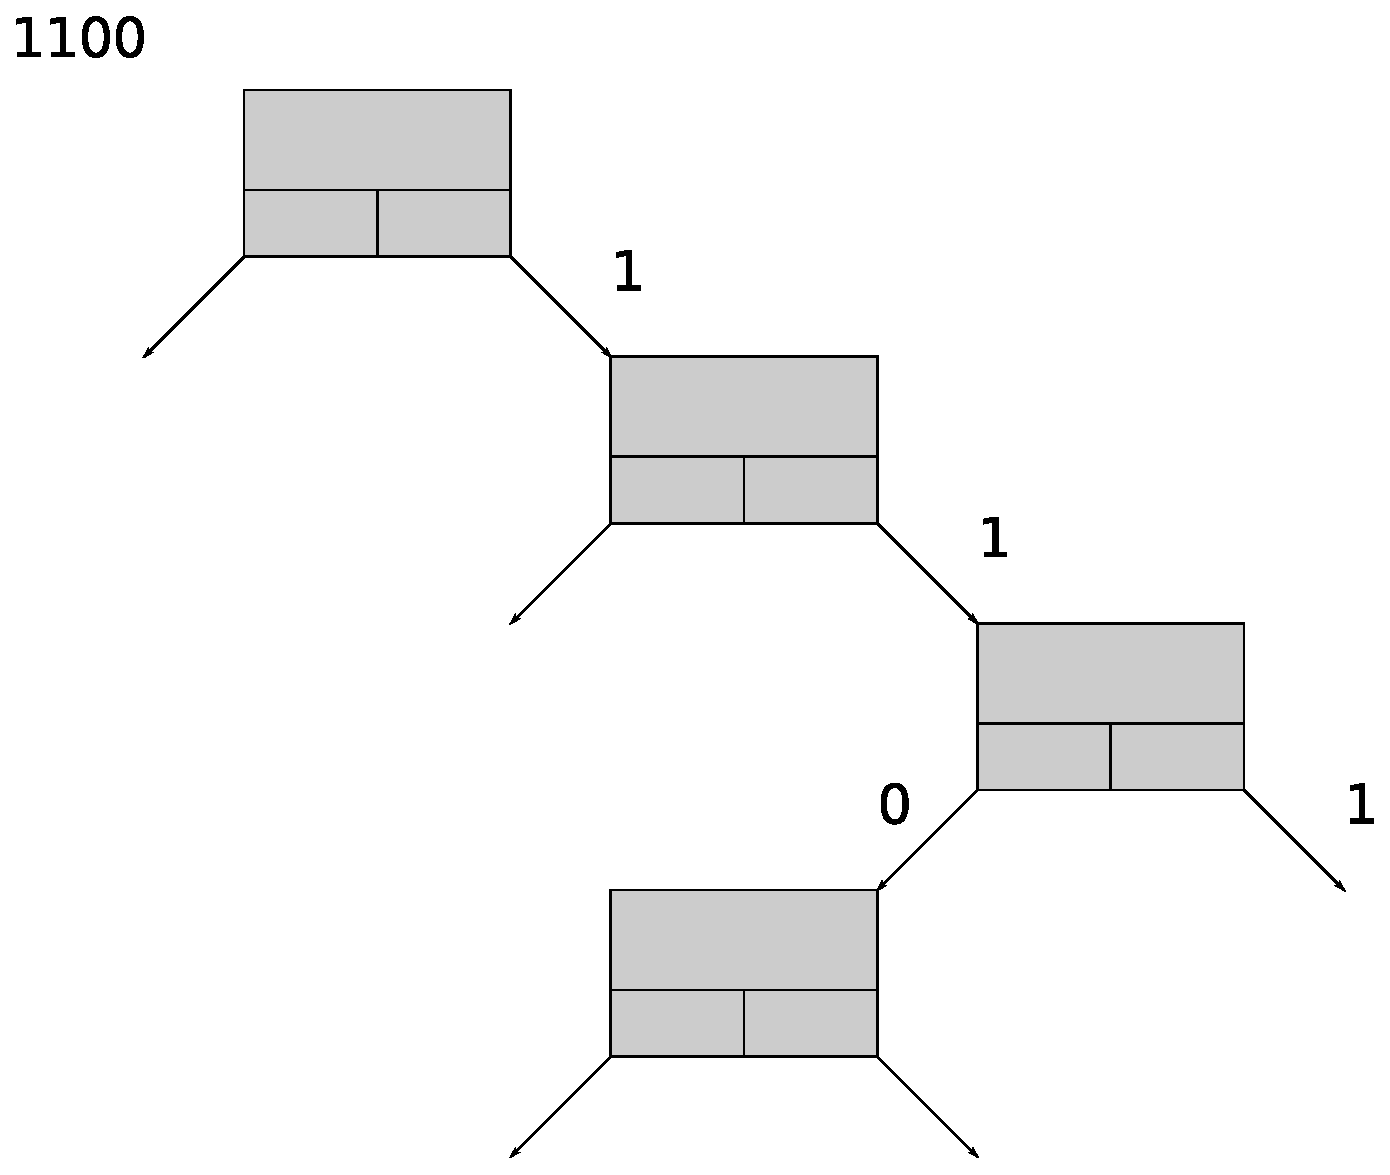
\includegraphics[scale=0.30]{figures/lluinsert04.eps} 
\end{frame}

\begin{frame}{Ejemplo inserción} 
\center	
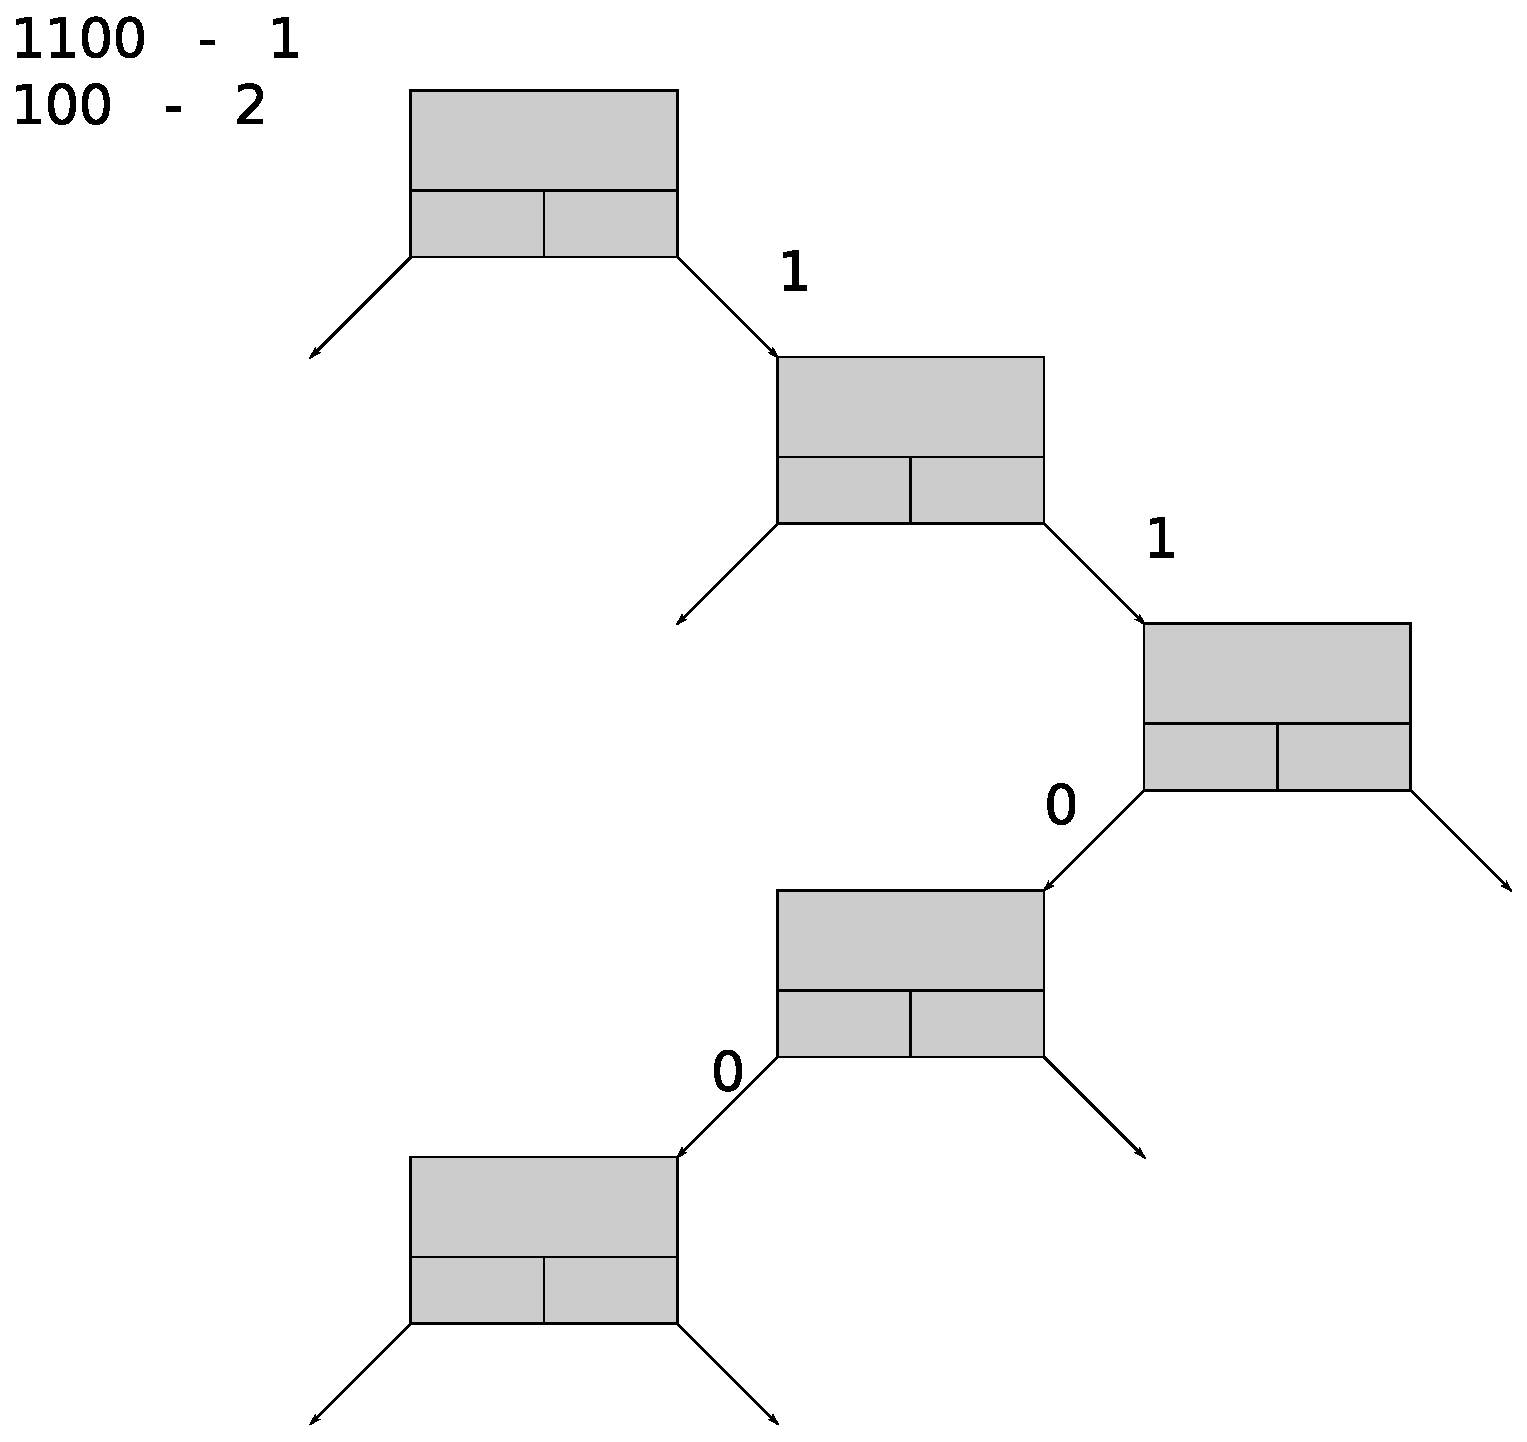
\includegraphics[scale=0.30]{figures/lluinsert05.eps} 
\end{frame}

\begin{frame}{Ejemplo inserción} 
\center	
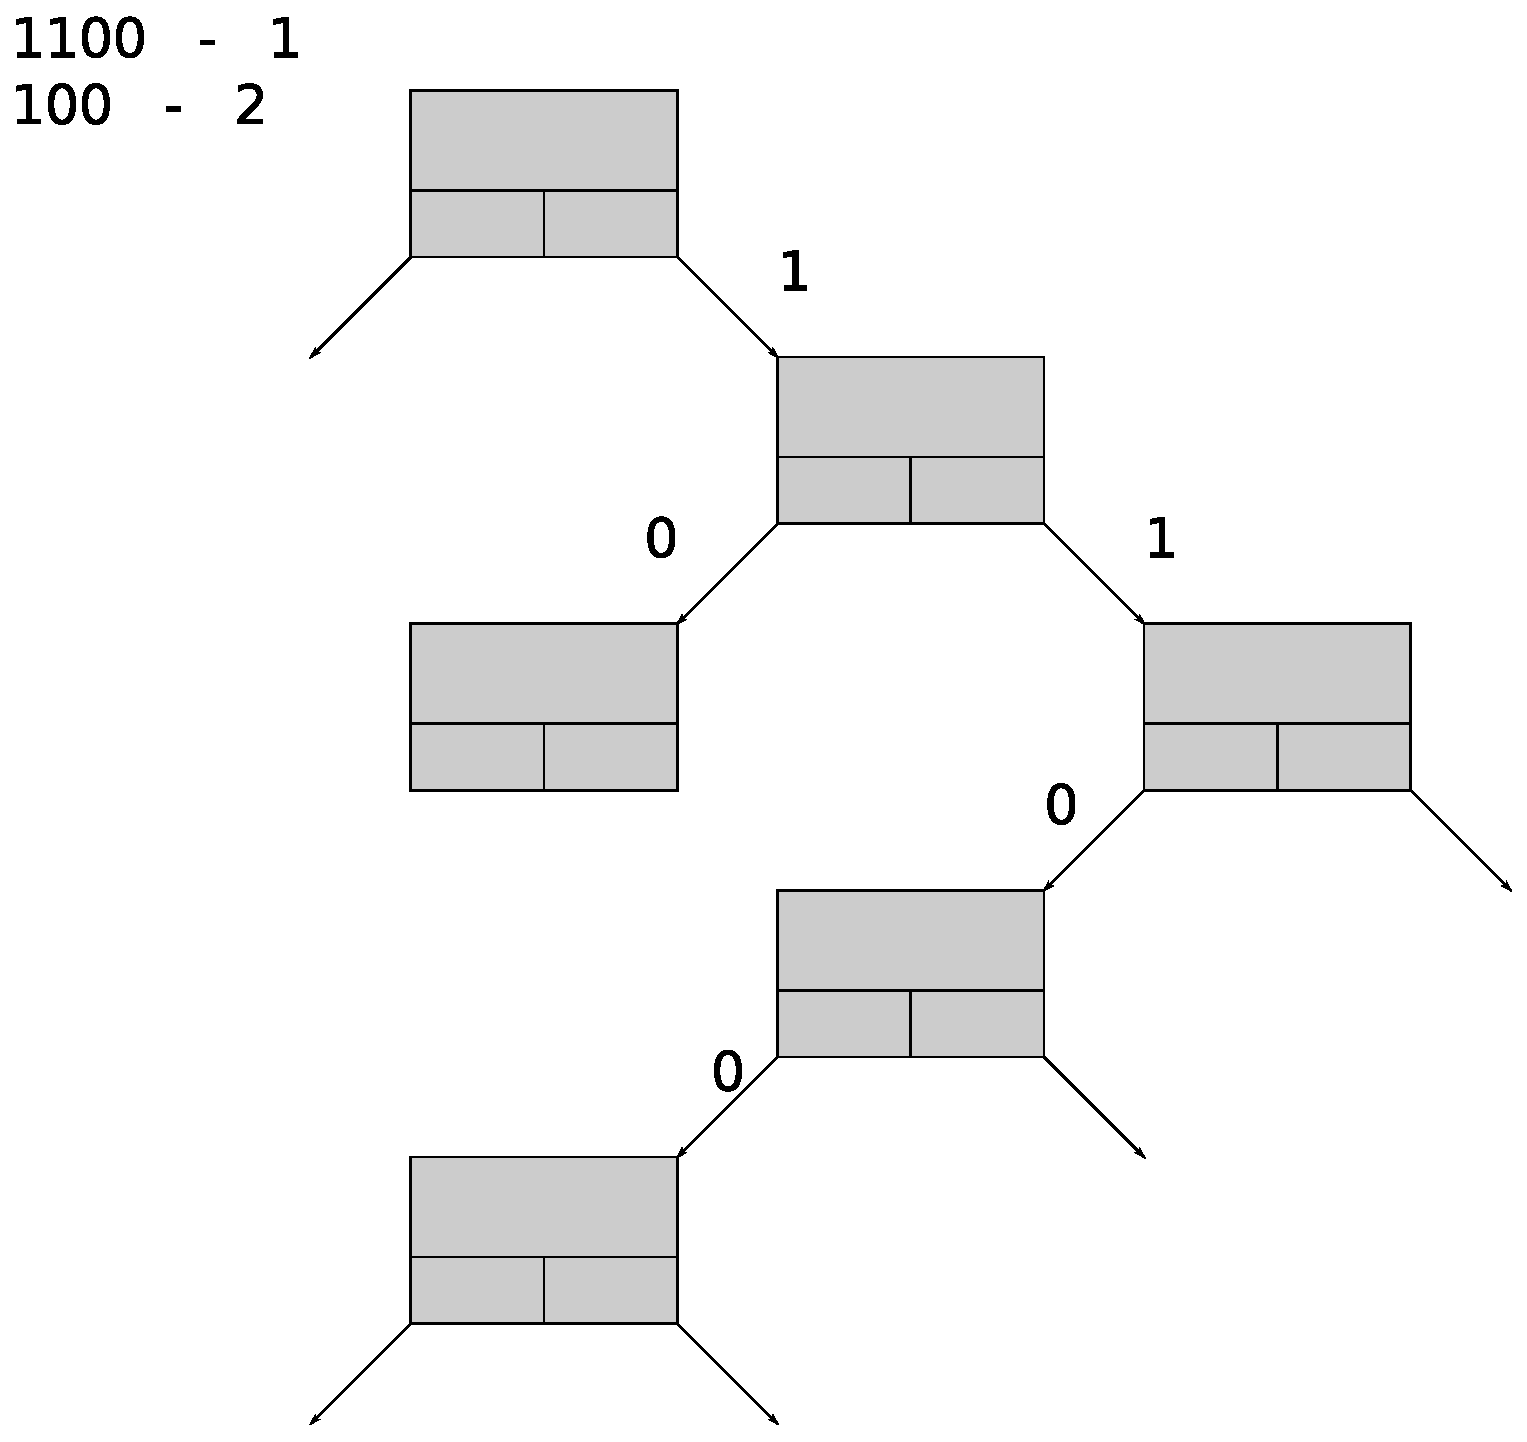
\includegraphics[scale=0.30]{figures/lluinsert06.eps} 
\end{frame}

\begin{frame}{Ejemplo inserción} 
\center	
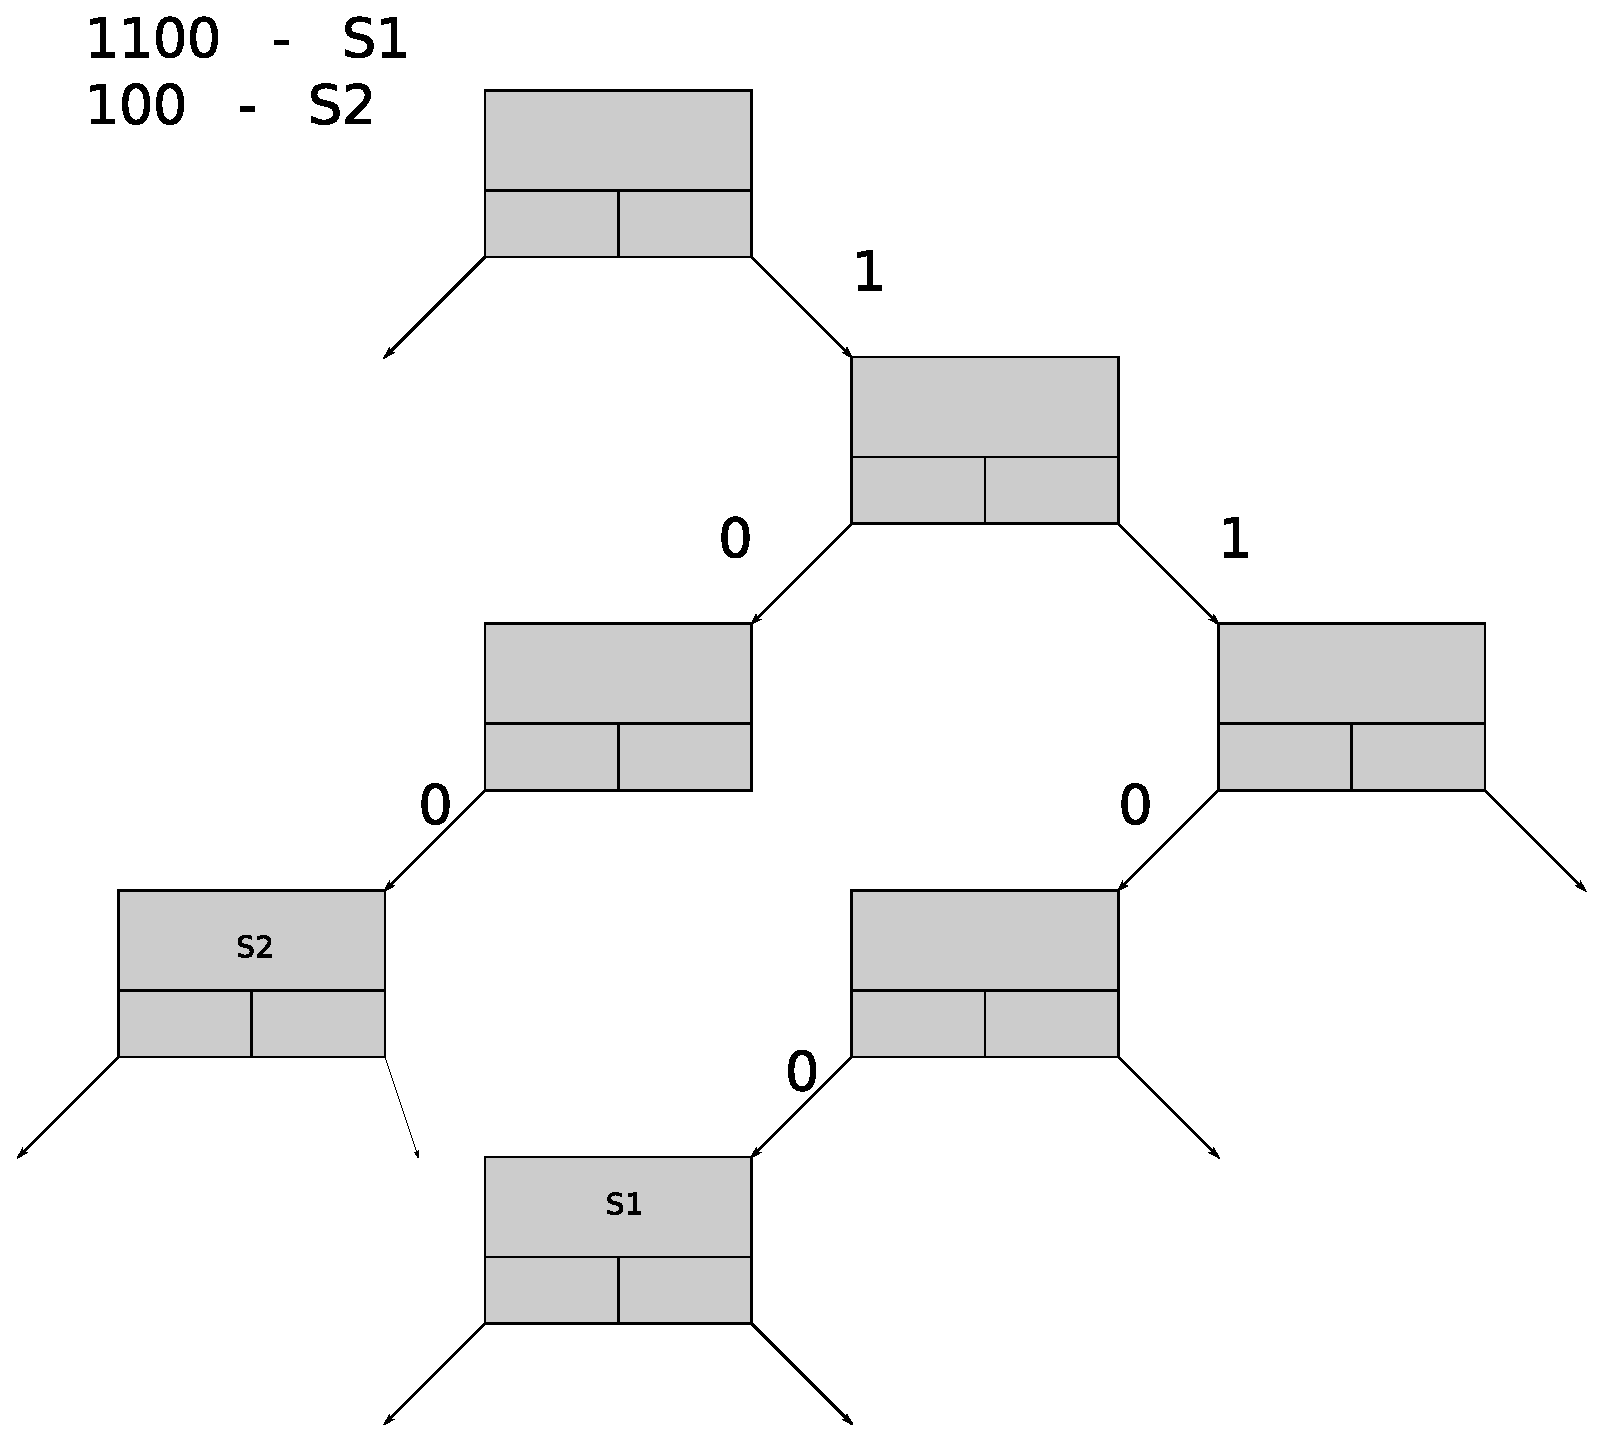
\includegraphics[scale=0.30]{figures/lluinsert07.eps} 
\end{frame}

\begin{frame}{Ejemplo inserción} 
\center	
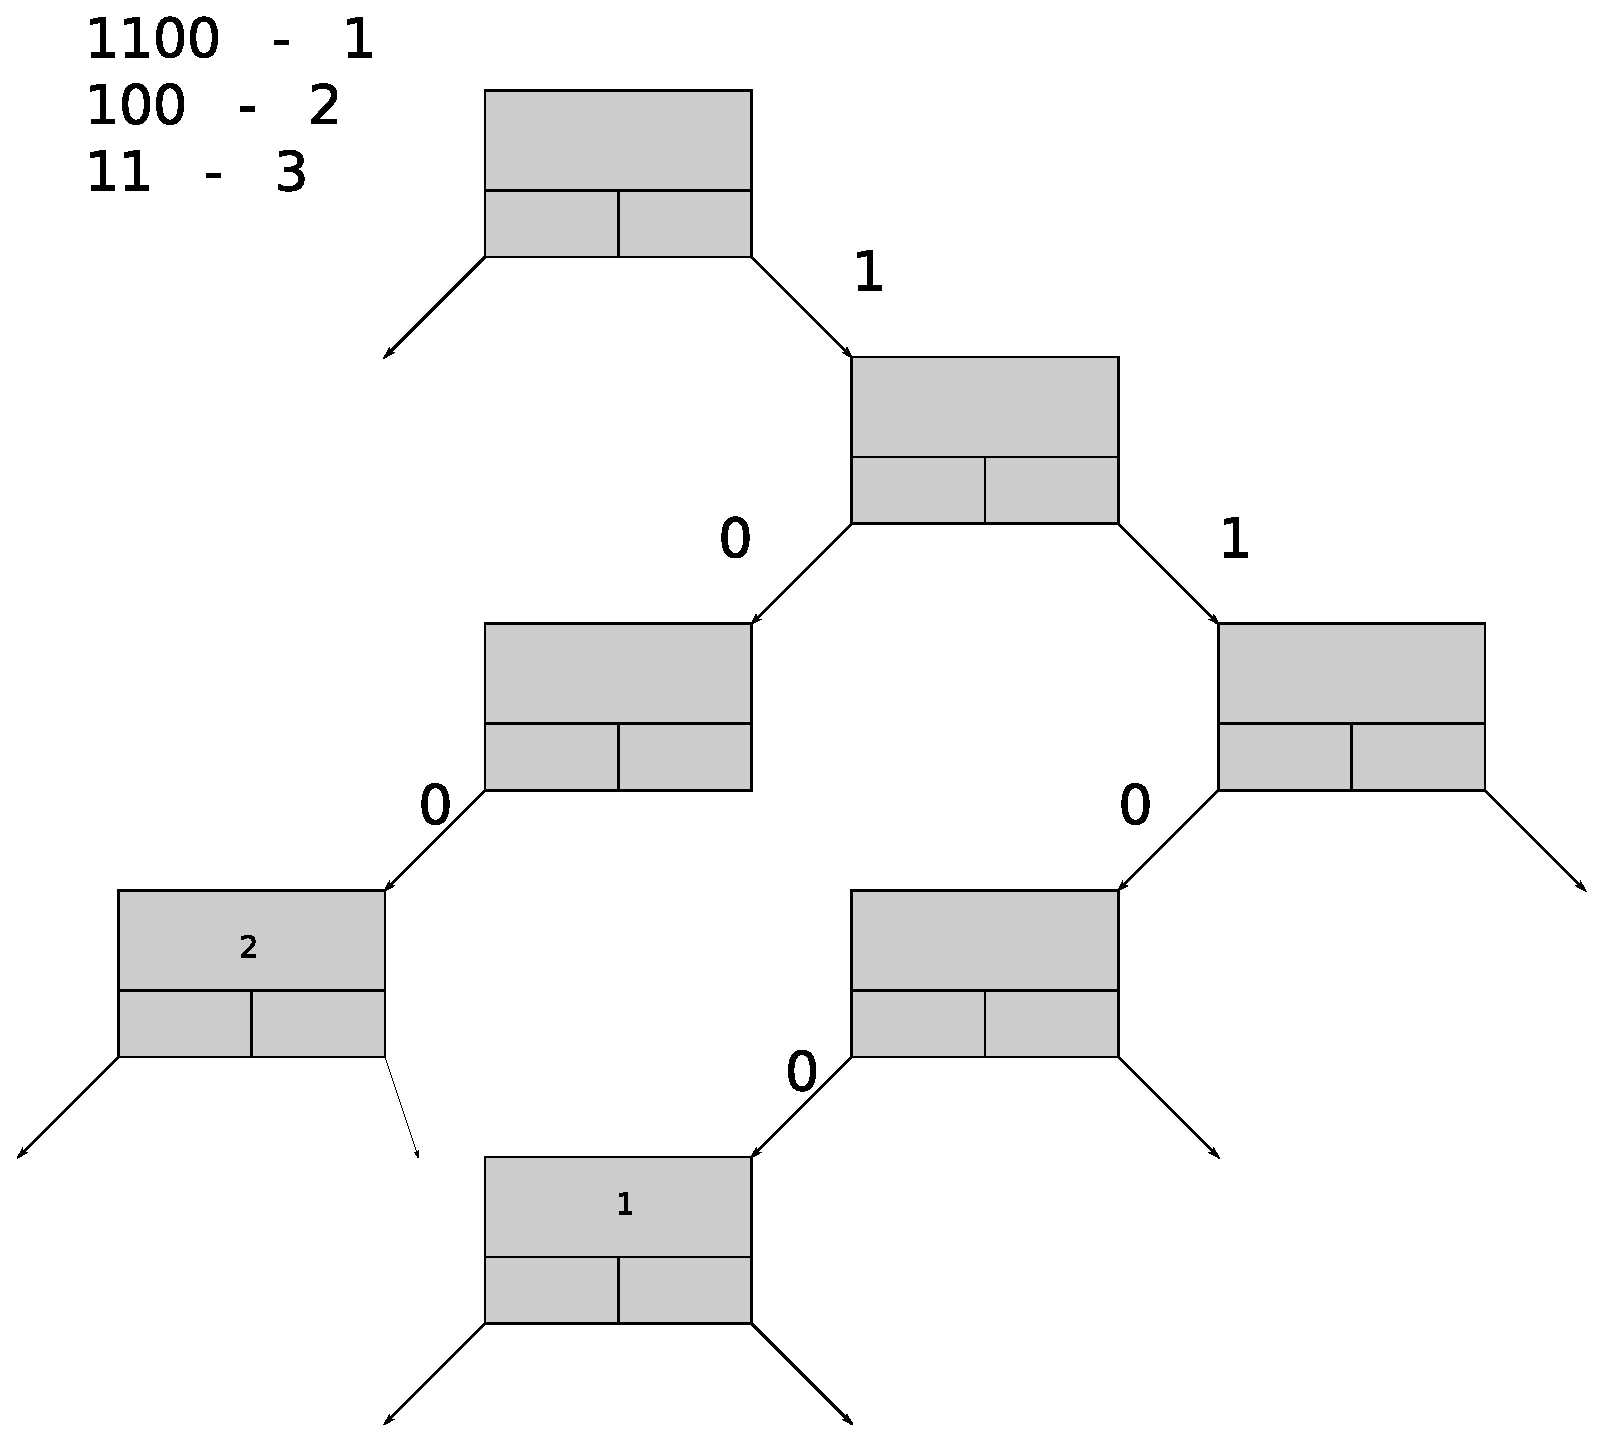
\includegraphics[scale=0.30]{figures/lluinsert08.eps} 
\end{frame}

\begin{frame}{Ejemplo inserción} 
\center	
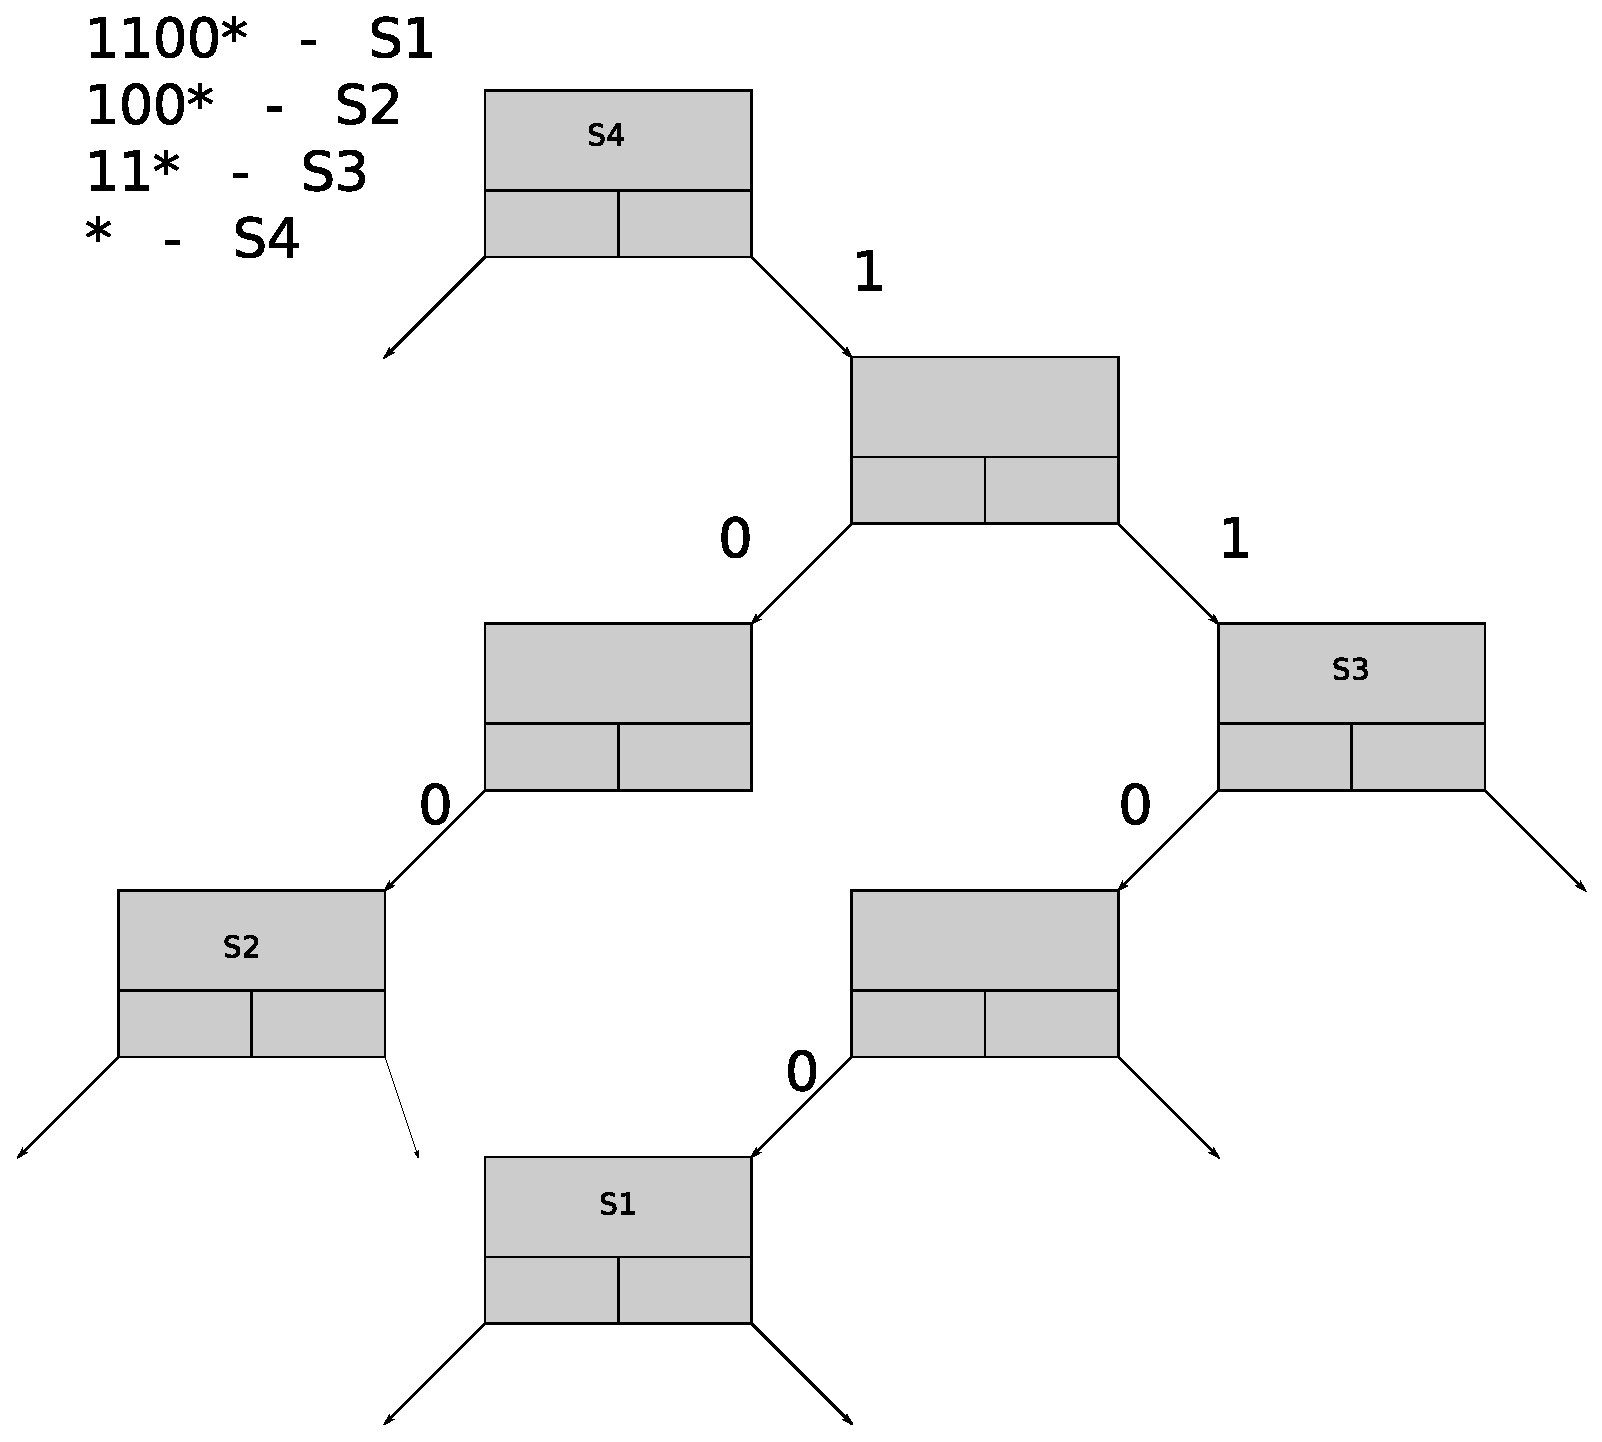
\includegraphics[scale=0.30]{figures/lluinsert09.eps} 
\end{frame}

\subsection{Caché}
%\begin{comment}
\begin{frame}{Caché}
  \begin{block}<+->{Caché} 	
    \begin{itemize}
      \scriptsize
     	\item Directa
	\item Tabla de 16 entradas
	\item Estructura \textit{HashEntry} (dirección, decisión, vacío)
	\item Colisiones se resuelven por reemplazo directo
     \end{itemize}
  \end{block}
  
  \begin{block}<+->{Funcionamiento} 	
    \begin{itemize}
      \scriptsize
     	\item Al tomar una dirección IP, chequear si el valor de decisión se encuentra en la caché
	\item Si se encuentra, retornar dicho valor.
	\item En otro caso, almacenarlo
     \end{itemize}
  \end{block}
\end{frame}

%\end{comment}


\subsection{ISR}
\begin{frame}{ISR}

  \begin{block}<+->{Elementos} 	
    \begin{itemize}
      \scriptsize
     	\item \textit{store\_array}: Buffer en el cual se van almacenando las palabras enviadas por Uplink. 3 enteros por fila (96 bits).
	\item \textit{i}: subíndice para moverse dentro del buffer
	\item \textit{flag}: se incrementa cada vez que se recibe una interrupción
	\item \textit{flag2}: se utiliza en conjunto con \textit{flag} controlar el bucle principal del programa. Se inicializa al mismo valor que \textit{flag}
     \end{itemize}
  \end{block}

  \begin{block}<+->{Funcionamiento} 	
    \begin{itemize}
      \scriptsize
     	\item El procesador recibe una interrupción.
	\item El valor leído se almacena en \textit{store\_array}, en la posición indicada por \textit{i}
	\item Se incrementan \textit{i} y \textit{flag}
	\item Se pierde la condición de igualdad entre \textit{flag} y \textit{flag2}, con lo cual se lleva a cabo la clasificación.
	\item Se asigna a \textit{flag2} el valor de \textit{flag}
	\item Uplink versión "Cabecera completa": Esperar 5° iteración.
	\item Uplink versión "Sólo IP destino": Trivial.
     \end{itemize}
  \end{block}
\end{frame}
  

\section{Integración}

\subsection{Plataforma}
\begin{frame}{Hardware}
  \begin{block}<+->{Placa de desarrollo DE2} 	
    \begin{itemize}
      \scriptsize
     	\item FPGA: Cyclone II EP2C35F672C6
	\item USB Blaster integrado, para configuración de FPGA
	\item Memoria: 8 MB SDRAM, 512 KB SRAM, 4 MB Flash
	\item Clock de 50 MHz
     \end{itemize}
  \end{block}

  \begin{block}<+->{FPGA Cyclone II EP2C35F672C6} 	
    \begin{itemize}
      \scriptsize
     	\item Elementos lógicos: 33216
	\item Bit totales de RAM: 483840
	\item Multiplicadores embebidos: 35
	\item PLLs: 4
	\item Cantidad máxima de pines definidos por el usuario: 475
     \end{itemize}
  \end{block}
\end{frame}


\begin{frame}{Microprocesadores - HardCores VS SoftCores}
   \begin{block}<+->{HardCores}	
    \begin{itemize}
	\scriptsize
     	\item Implementados de forma permanente en el silicio.
	\item Gran rendimiento a expensas de altos costos en FPGA.
	\item Tendencia actual: HardCore incluido.
	\item No disponible en FPGA de este trabajo.
    \end{itemize}	
  \end{block}
  
  \begin{block}<+->{SoftCores}	
    \begin{itemize}
	\scriptsize
     	\item Definidos a nivel de descripción de hardware.
	\item Instanciados en la lógica de la FPGA.
	\item Implementaciones libres y propietarias.
    \end{itemize}	
  \end{block}
\end{frame}

\subsection{NIOS II}
\begin{frame}{Microprocesador NIOS II}
\center
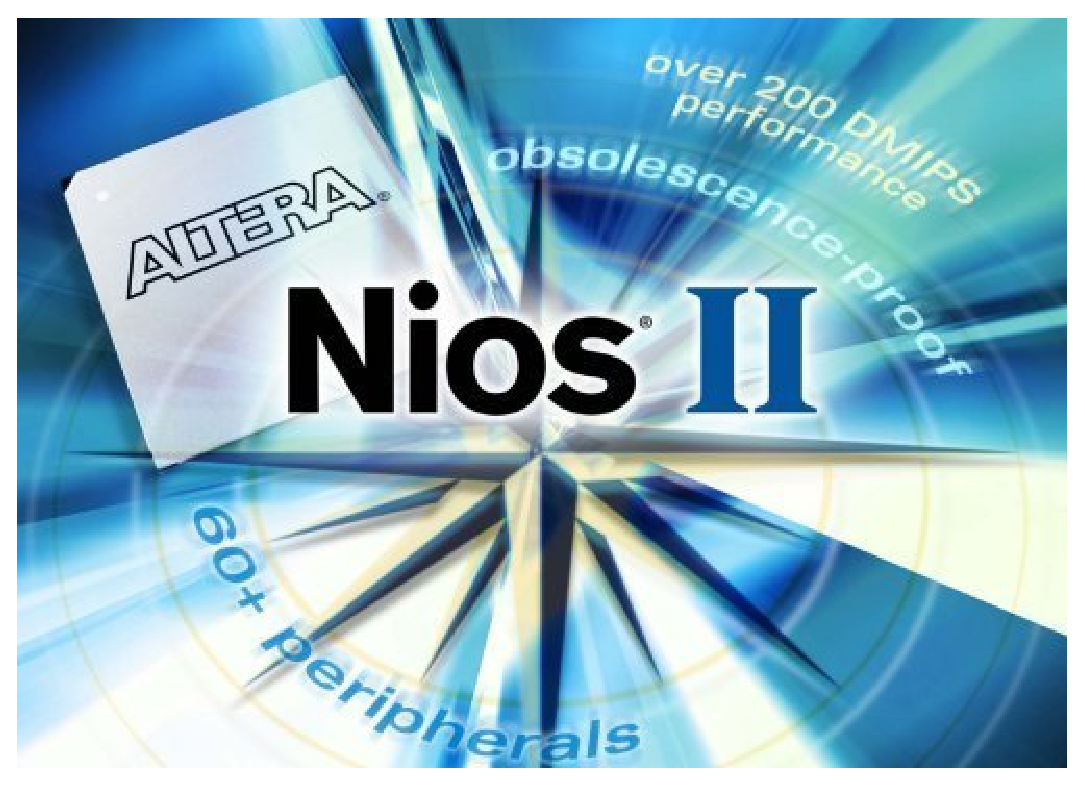
\includegraphics[scale=0.20]{figures/nios2.eps}
   \begin{block}<+->{NIOS II}	
    \begin{itemize}
	\scriptsize
     	\item Procesador RISC de 32 bits de propósito genera diseñado específicamente para la familia de FPGAs de Altera.
	\item Set de instrucciones, bus de datos y espacio de direcciones de 32 bits.
	\item Soporte de hasta 32 interrupciones.
	\item Entorno de desarrollo de software basado en GNU C/C++ integrado a Eclipse.
	\item Integración con SignalTap® II, el analizador de lógica embebida de Altera permitiendo el análisis  de todas las señales presentes en la FPGA.
	\item Set de instrucciones compatible entre todos las versiones del procesador Nios II.
	\item Multiplicación y división en una sola instrucción de 32 x 32 produciendo un resultado de 32-bits.
	\item Se utilizará la versión que ofrezca una mejor performance
    \end{itemize}	
  \end{block}
\end{frame}

\subsection{Herramientas}
\begin{frame}{Herramientas de Desarrollo}
\begin{block}<+->{Quartus} 
	
    \begin{itemize}
      \scriptsize
     	\item IDE de Altera
	\item Incluye editor de textos y herramientas para síntesis
	\item Lenguaje HDL utilizado: Verilog HDL
    \end{itemize} 
	\center
	
\includegraphics[scale=0.10]{figures/Quartus.eps}  
  \end{block}
  \begin{block}<+->{Eclipse IDE for NIOS}   
	
    \begin{itemize}
      \scriptsize
     	\item Versión de la IDE Eclipse adaptada para trabajar con el microprocesador NIOS II
	\item Lenguajes utilizados: C,C++
    \end{itemize}
	\center	
	
\includegraphics[scale=0.10]{figures/eclipse.eps}  	
  \end{block}
\end{frame}

\begin{frame}{Sistema Embebido}
\center
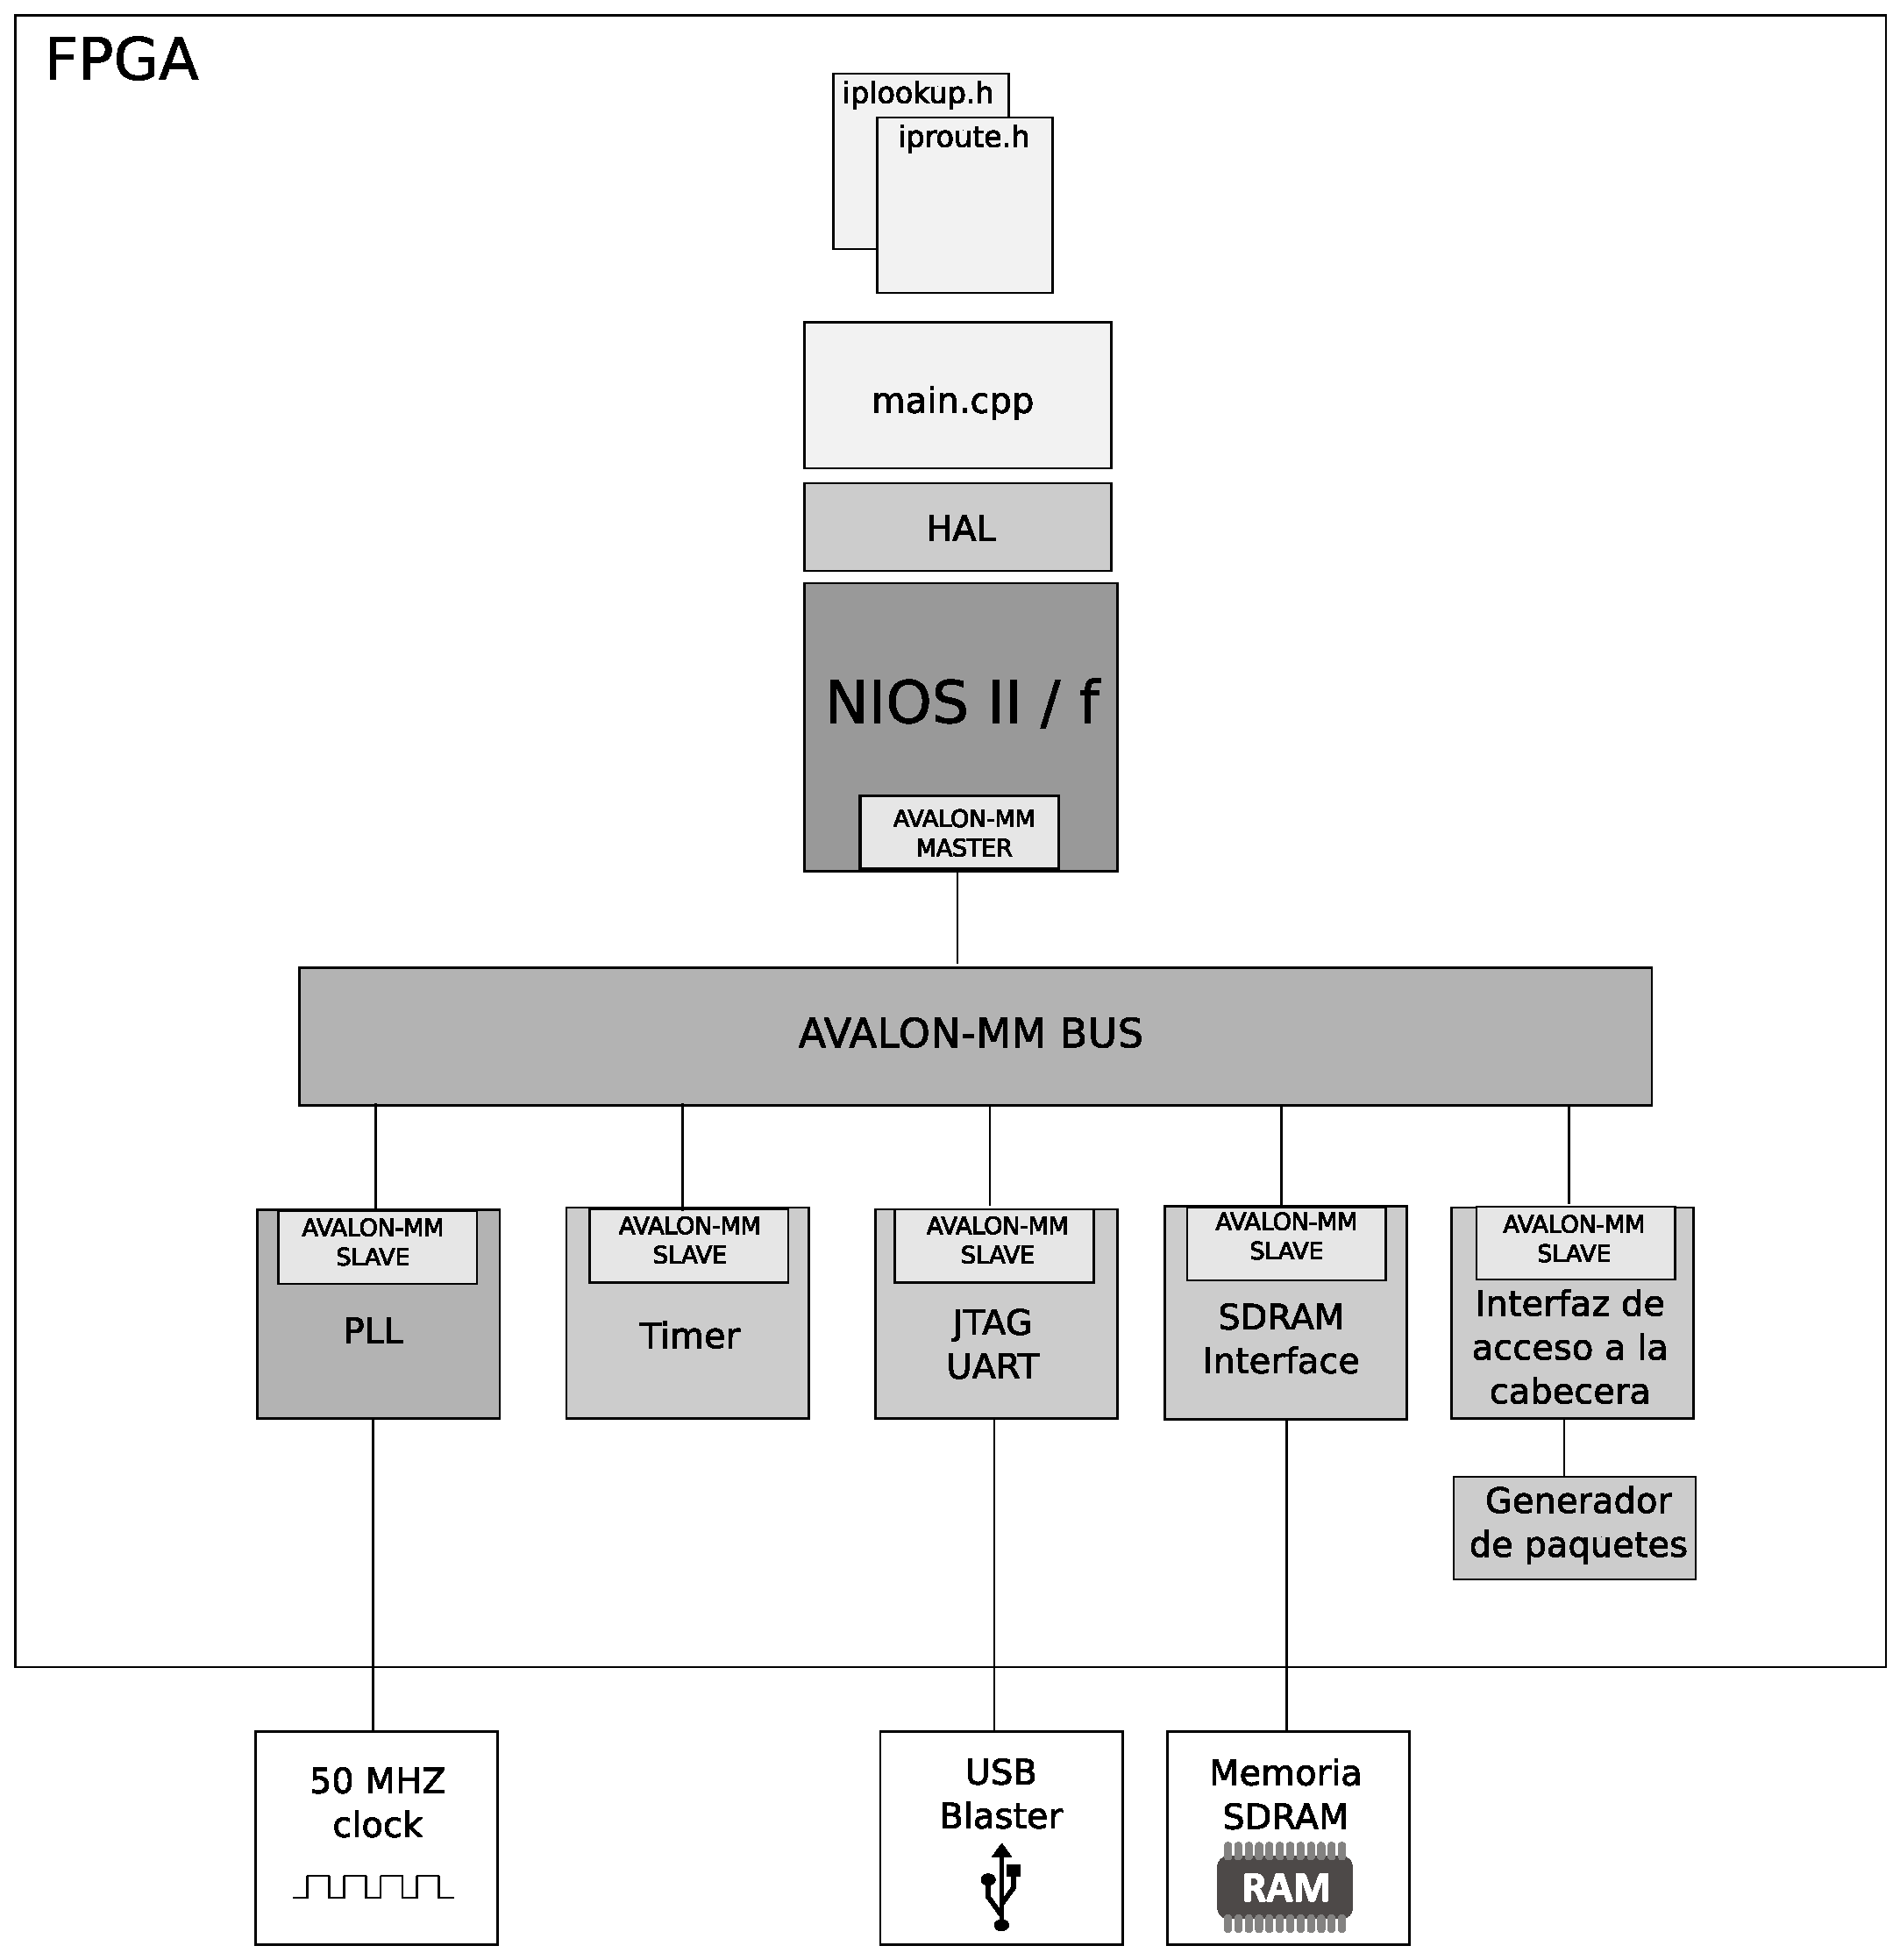
\includegraphics[scale=0.20]{figures/sistema.eps}
   

\end{frame}


\subsection{Verificación}
\begin{frame}{Uso de la FPGA}

	\center	
	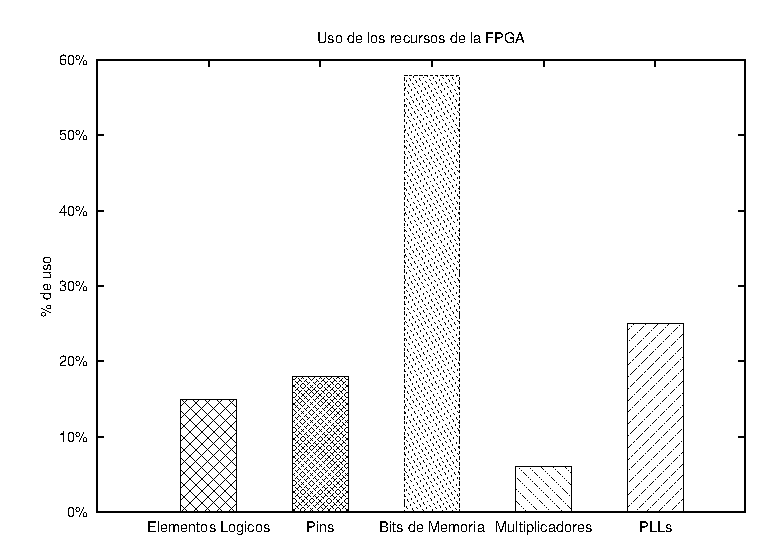
\includegraphics[scale=0.30]{figures/fpga.eps}  
	

   \begin{block}<+->{Recursos totales utilizados}	
    \begin{itemize}
	\scriptsize
     	\item Elementos lógicos: 4983 (15\% del total).
	\item Bits de RAM: 280627.
	\item Multiplicadores embebidos: 2 (de 35).
	\item PLLs: 1 (de 4).
	\item Pines definidos: 86 (de 475).
	\item Remanente importante de recursos -> Posibilidad de ampliar las funcionalidades del sistema (ej, uso de multicores).
    \end{itemize}	
  \end{block}


\end{frame}


\section{Resultados}
%\subsection{Introducción}
\begin{frame}{Introducción}
	\begin{block}<+->{Resultados}  
	 \begin{itemize}	
		\item Se presentan los datos obtenidos de la ejecución del proyecto bajo ciertas condiciones representativas. 
		\item Primero se estudiara el tiempo de respuesta de los algoritmos de manera individual, 
		\item En segundo lugar,  el rendimiento en la configuración mas simple
		\item Luego el sistema completo bajo condiciones varias
		\item Por ultimo el estudio de la mejora introducida por el uso de la cache. 
		\item Para la obtencion de los datos que corresponden al sistema completo se utilizo el Script Python/Bash.
	\end{itemize}
  \end{block}
\end{frame}

\subsection{Stress de Software}
\begin{frame}{Stress de Software}
\begin{block}<+->{Stress de Software}   
    \begin{itemize}
      \scriptsize
     	\item Retardo de búsqueda en función de la posición en la tabla de enrutamiento.
     	\item Independiente al modulo extracto de cabeceras.
	\item En el eje de las abscisas se expresa la ubicación en una tabla de 100 elementos del prefijo mas largo.
	\item En las ordenadas se puede observar el tiempo de búsqueda en ciclos de reloj.
	\item LLU: Retardo depende de la posición en la lista.
	\item UTL: Retardo depende de la longitud del prefijo.
    \end{itemize}
  \end{block}
\end{frame}

\begin{frame}{Caso algoritmos únicamente} 
\center	
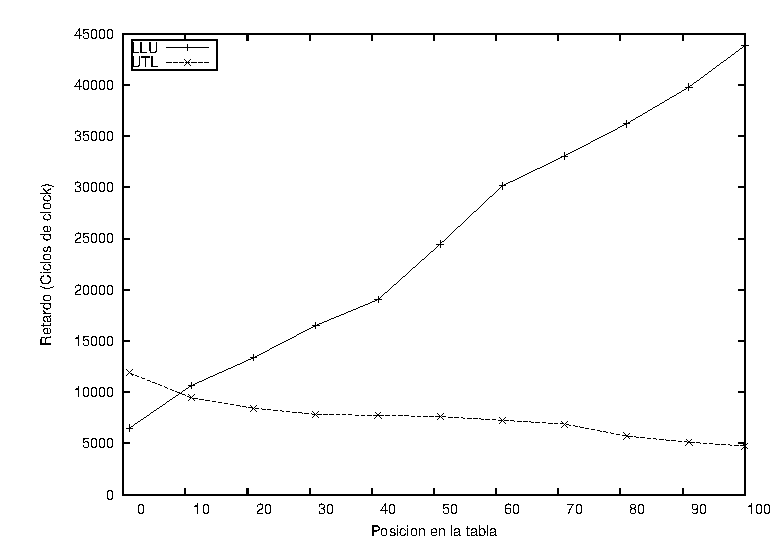
\includegraphics[scale=0.70]{figures/llu-utlsof.eps} 
\end{frame}

\subsection{Caso loopback}

\begin{frame}{Caso loopback} 
\begin{block}<+->{Caso loopback}   
    \begin{itemize}
      \scriptsize
     	\item Finalidad: encontrar los limites superiores del sistema
     	\item el software solo se limita a recibir los datos e inmediatamente después confirma el procesamiento y envía los resultados de regreso al hardware
	\item Pruebas correspondientes para las dos versiones de Uplink
	\item Abscisas: cantidad de paquetes por segundo
	\item Ordenadas: cantidad de paquetes perdidos en valores porcentuales
	\item Se procesó una cantidad constante de paquetes, 9000, y luego se contrasto este valor con un contador global que el Generador estampa en la ultima palabra de cada paquete
    \end{itemize}
  \end{block}
\end{frame}

\begin{frame}{Caso loopback} 
\center	
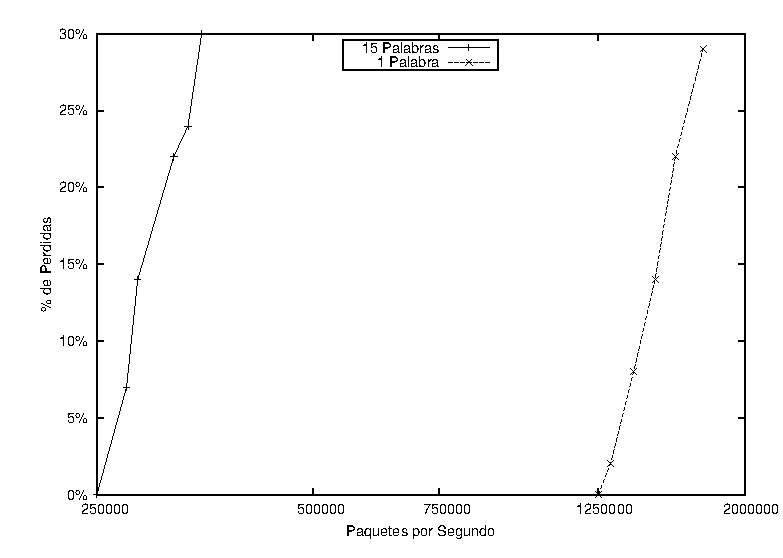
\includegraphics[scale=0.70]{figures/loop.eps} 
\end{frame}

\subsection{Implementación completa}
\begin{frame}{Implementación completa} 
 \begin{block}<+->{Implementación completa}   
    \begin{itemize}
      \scriptsize
     	\item Se consideraran tres puntos en las curvas que indican los tiempos de accesos del algoritmos
     	\item Un punto mínimo que corresponde al menor tiempo de acceso
	\item Un punto promedio que ejercita 10 entradas equidistantes a lo largo de la tabla
	\item punto máximo que indica el peor tiempo de acceso posible para un algoritmo dado	
    \end{itemize}
  \end{block}
\end{frame}

\begin{frame}{Implementación completa: LLU (mínimo)} 
\center	
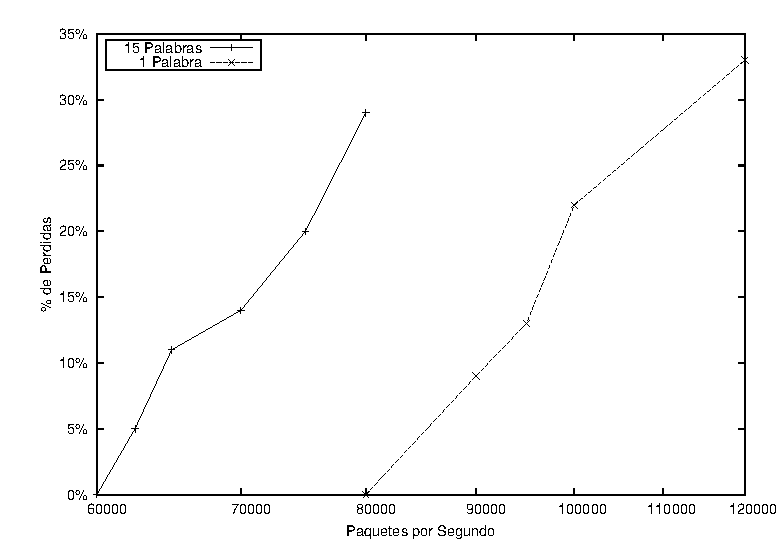
\includegraphics[scale=0.70]{figures/llumin.eps} 
\end{frame}


\begin{frame}{Implementación completa: LLU (promedio)} 
\center	
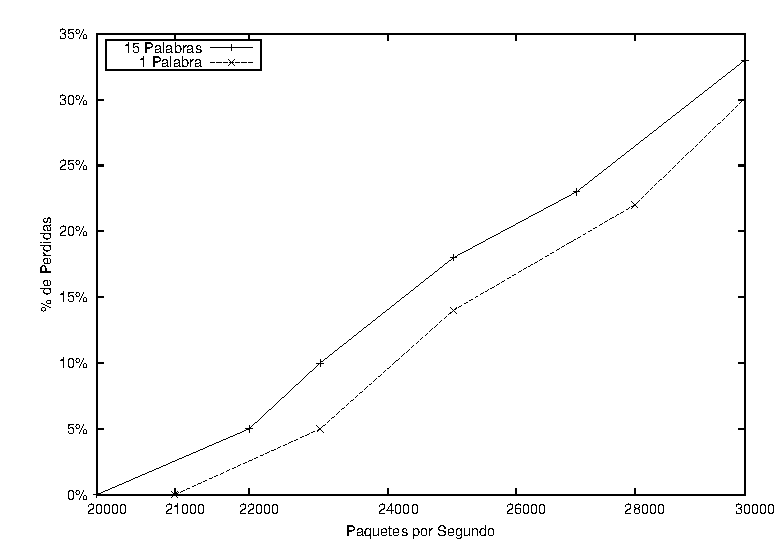
\includegraphics[scale=0.70]{figures/lluprom.eps} 
\end{frame}


\begin{frame}{Implementación completa: LLU (máximo)} 
\center	
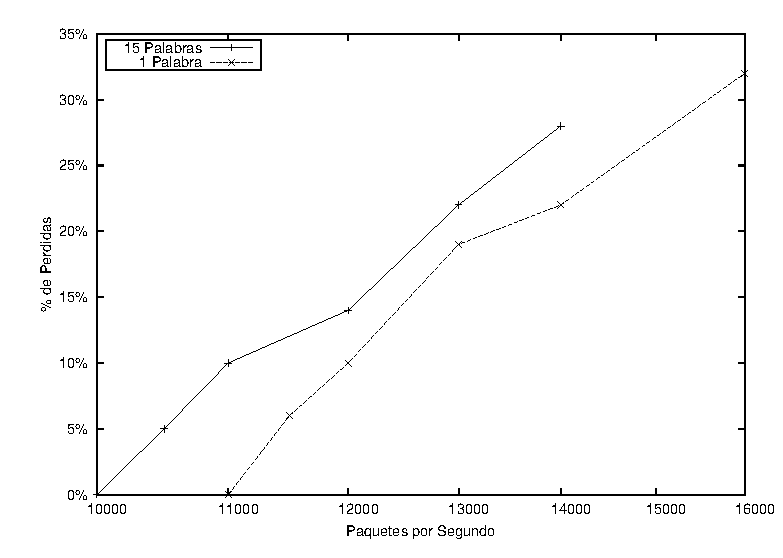
\includegraphics[scale=0.70]{figures/llumax.eps} 
\end{frame}

\begin{frame}{Implementación completa: LLU} 
 \begin{block}<+->{LLU}   
    \begin{itemize}
      \scriptsize
     	\item La diferencia en la cantidad de paquetes que pueden ser transmitidos sin errores en el mejor caso entre el modulo que envía una palabra al procesador y el que envía toda la cabecera, es considerable
     	\item A medida que aumenta la profundidad de búsqueda en la tabla estos valores convergen
	\item Resultado esperable, ya que para accesos muy lentos a la tabla el retardo introducido por el Hardware se vuelve despreciable
    \end{itemize}
  \end{block}
\end{frame}

\begin{frame}{Implementación completa: UTL (mínimo)} 
\center	
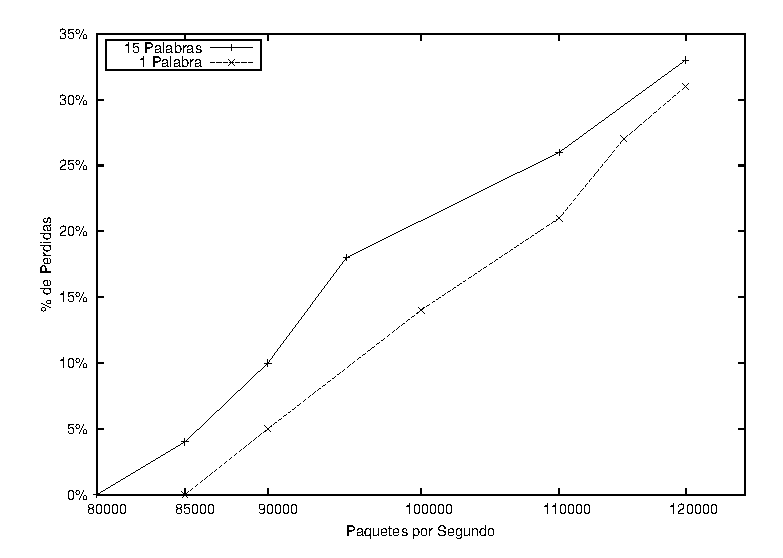
\includegraphics[scale=0.70]{figures/utlmin.eps} 
\end{frame}


\begin{frame}{Implementación completa: UTL (promedio)} 
\center	
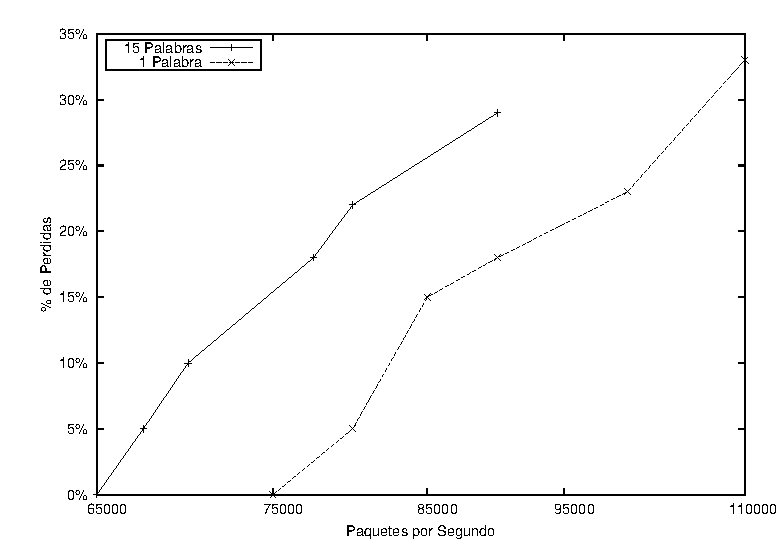
\includegraphics[scale=0.70]{figures/utlprom.eps} 
\end{frame}


\begin{frame}{Implementación completa: UTL (máximo)} 
\center	
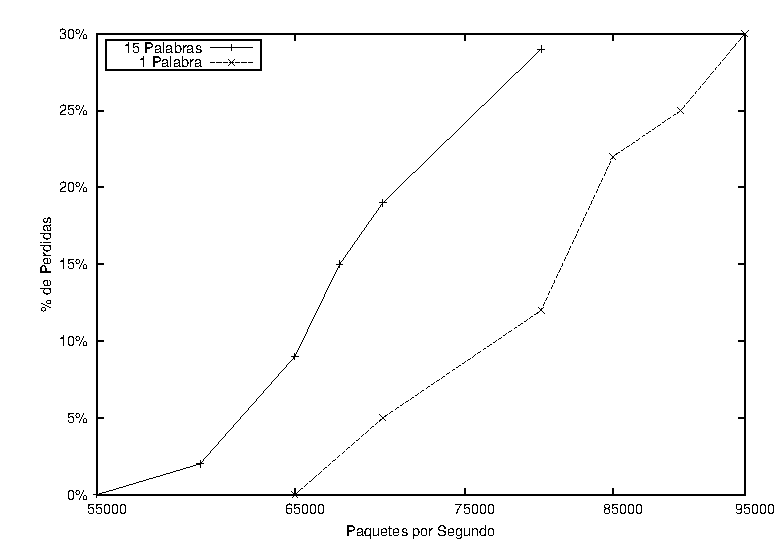
\includegraphics[scale=0.70]{figures/utlmax.eps} 
\end{frame}

\begin{frame}{Implementación completa: UTL} 
 \begin{block}<+->{UTL}   
    \begin{itemize}
      \scriptsize
     	\item Existe una menor diferencia entre la máxima cantidad de paquetes que pueden ser transmitidos sin error en cada uno de los 3 puntos elegidos
     	\item También la diferencia entre enviar el paquete entero y solo la IP destino se reduce
	\item Cuando el tiempo de acceso es uniforme el impacto de la mejoras del Hardware tiende a ser menor
    \end{itemize}
  \end{block}
\end{frame}

\subsection{Comparativa inter-algortimos}
\begin{frame}{Comparativa inter-algortimos} 
\center	
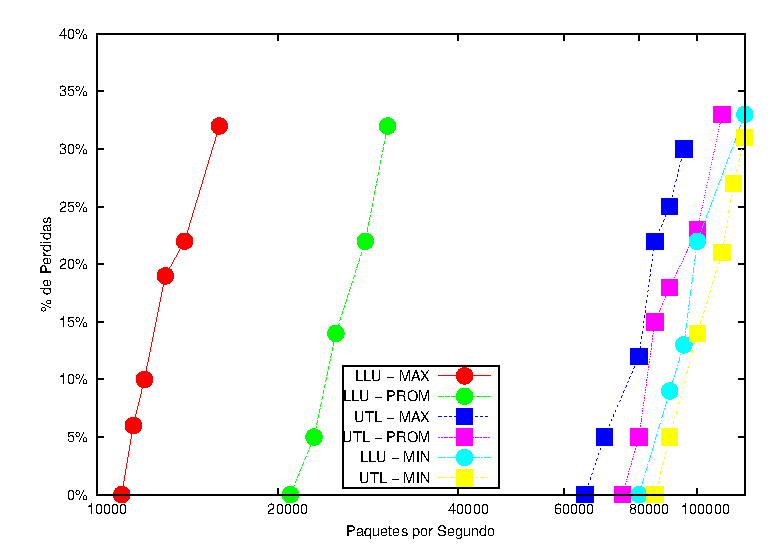
\includegraphics[scale=0.70]{figures/lluvsutl.eps} 
\end{frame}

\section{Conclusiones}
\begin{frame}{Conclusiones} 
\begin{block}<+->{Conclusiones}   
    \begin{itemize}
      \scriptsize
     	\item Factibilidad de implementación.
     	\item HW -> Velocidad de procesamiento.
     	\item SW -> Escalabilidad.
     	\item Complejidad -> Implementación del SoC, curva de aprendizaje de las herramientas.
     	\item Modularidad -> Portabilidad.
     	\item Integración de los 3 ejes de la carrera.      	
    \end{itemize}
  \end{block}
  \begin{block}<+->{Trabajos futuros.}   
    \begin{itemize}
      \scriptsize
     	\item Clasificación multidimensional.
     	\item Optimización de código para NIOS II.
     	\item Portar el sistema a otras plataformas.
     	\item Caché por HW.
     	\item Mecanismos de actualización automática de la tabla de ruteo.
     	\item Complementación con otros trabajos.     	
    \end{itemize}
  \end{block}
\end{frame}

\end{document}
